
%%%%%%%%%%%%%%%%%%%%%%% file typeinst.tex %%%%%%%%%%%%%%%%%%%%%%%%%
%
% This is the LaTeX source for the instructions to authors using
% the LaTeX document class 'llncs.cls' for contributions to
% the Lecture Notes in Computer Sciences series.
% http://www.springer.com/lncs       Springer Heidelberg 2006/05/04
%
% It may be used as a template for your own input - copy it
% to a new file with a new name and use it as the basis
% for your article.
%
% NB: the document class 'llncs' has its own and detailed documentation, see
% ftp://ftp.springer.de/data/pubftp/pub/tex/latex/llncs/latex2e/llncsdoc.pdf
%
%%%%%%%%%%%%%%%%%%%%%%%%%%%%%%%%%%%%%%%%%%%%%%%%%%%%%%%%%%%%%%%%%%%


\documentclass[a4paper]{llncs}

\usepackage{amssymb}
\setcounter{tocdepth}{3}
\usepackage{graphicx}
\usepackage{fixltx2e}
\usepackage{authblk}
\usepackage{url}
\usepackage{wrapfig}
\usepackage{times}
\usepackage{verbatim}


\usepackage[table]{xcolor} 
\usepackage{booktabs}
\usepackage{tikz}
\def\checkmark{\tikz\fill[scale=0.4](0,.35) -- (.25,0) -- (1,.7) -- (.25,.15) -- cycle;} 
\usepackage{algorithm}
\usepackage[noend]{algpseudocode}
\usepackage{color}

\usepackage{titlesec}
\usepackage{enumitem}
\usepackage{verbatim}


\urldef{\mailsa}\path|{alfred.hofmann, ursula.barth, ingrid.haas, frank.holzwarth,|
\urldef{\mailsb}\path |anna.kramer, leonie.kunz, christine.reiss, nicole.sator,|
\urldef{\mailsc}\path|erika.siebert-cole, peter.strasser, lncs}@springer.com|    
\newcommand{\keywords}[1]{\par\addvspace\baselineskip
\noindent\keywordname\enspace\ignorespaces#1}


\begin{document}

\newcommand{\isa}{\textit{is-a}}
\newcommand{\eulerx}{\textsc{Euler/x}}
\newcommand{\RRR}{\ensuremath{\mathsf{R}_{32}}}
\newcommand{\theName}{\textit{CactusTree}}
\newcommand{\theNames}{\textit{CactusTrees}}

\mainmatter  % start of an individual contribution

% first the title is needed
\title{A User Study of Techniques for Visualizing Structure and Connectivity in Hierarchical Datasets}

% a short form should be given in case it is too long for the running head
\titlerunning{A User Study of Techniques for Visualizing Structure and Connectivity in Hierarchical Datasets}

% the name(s) of the author(s) follow(s) next
%
% NB: Chinese authors should write their first names(s) in front of
% their surnames. This ensures that the names appear correctly in
% the running heads and the author index.
%
%\author{Tuan Nhon Dang
%\and Nico Franz \and Bertram Lud\"ascher \and Angus Graeme Forbes}


\author[1]{Tommy Dang}
\author[2]{Paul Murray}
\author[3]{Ronak Etemadpour}
\author[4]{Angus G. Forbes}
\affil[1]{Texas Tech University, Lubbock, TX, USA}
\affil[2]{The New York Times’ Interactive News Desk, New York, NY, USA}
\affil[3]{City College, CUNY, New York, NY, USA}
\affil[4]{University of California, Santa Cruz, CA, USA}

%
\authorrunning{Tommy Dang, Paul Murray, Ronak Etemadpour, and Angus G. Forbes}
%\authorrunning{}
% (feature abused for this document to repeat the title also on left hand pages)

% the affiliations are given next; don't give your e-mail address
% unless you accept that it will be published

%
% NB: a more complex sample for affiliations and the mapping to the
% corresponding authors can be found in the file "llncs.dem"
% (search for the string "\mainmatter" where a contribution starts).
% "llncs.dem" accompanies the document class "llncs.cls".
%



\toctitle{Lecture Notes in Computer Science}
\tocauthor{Authors' Instructions}


\maketitle

\begin{abstract}
Many tree layouts have been created for presenting hierarchical data. However, layouts optimized for some tasks are not adequate for others. In this paper, we focus on identifying tree structures and cross-links generated by hierarchical edge bundling. Our key contribution is the introduction of descriptive features that can be used to characterize trees in terms of their structural and connective qualities. We present a user study with 14 subjects that provides an evaluation of our approach in comparison to other popular tree visualization techniques. The results of the study indicate which techniques are more effective for visual analysis tasks that involve identifying and comparing tree and subtree structures and/or visualizing connections using hierarchical edge bundling.

\keywords{Hierarchical edge bundling, tree layouts, user evaluation.}
\end{abstract}

\section{Introduction}
%Trees are one of the most fundamental data types. However, existing tree layout techniques are not always adequate for many real-world datasets. Layouts that aim to visually simplify complex trees can also make it difficult to perform common tasks, such as finding nodes or subtrees with particular characteristics. In addition to facilitating reasoning about hierarchical relationships, many application domains require the presentation of non-hierarchical relations between data items. %For example, in the domains of systems biology and molelcular biology, researchers analyze intracellular signaling pathways that can be composed of nested sets of biomolecules (i.e., proteins and protein complexes). When displaying signaling pathways it can also be important to clearly show how particular biomolecules influence or are influenced by others~\cite{Dang2015ReactionFlow}. That is, it may be necessary to highlight relevant interconnections between trees or subtrees while at the same time making sure not to obscure the hierarchical information in the tree. Similarly, in the domain of biodiverstiy informatics, the hierarchical structure of a phylogenic tree can usefully be overlaid with additional information that connects nodes in the tree in order to show, for instance, properties of a food web~\cite{OneZoom2012}. Many other examples can be found in real-world datasets.
An important consideration in visualizing complex hierarchical data, such as biological pathways, phylogenic trees, and ontological taxonomies, is clearly showing how particular elements relate to or are influenced by other elements. That is, it can be necessary to highlight relevant interconnected subtrees with a particular directionality, while at the same time making sure not to obscure the structure and hierarchical information represented by the tree. Many existing approaches~\cite{Bach2016confluentgraphs,Holten2009StudyHEB,McGee2012StudyHEB} investigate the use of hierarchical edge bundling techniques~\cite{HierarchicalEdgeBundles2006}, and our previous work also introduces \theName{}~\cite{Dang2017CactusTrees}, an interactive technique for visualizing the structure and connectivity in nested trees. %\theName{} was inspired by our work in creating biological pathways visualizations that enable a range of visual analytics tasks.


In this paper, we explore the effective use of tree layouts to support hierarchical structure recognition and to minimize ambiguity introduced by bundling cross-edges (also called non-hierarchical connections/links). A user study that uses both real-world and synthetic datasets validates the effectiveness of our approach. Additionally, the results of our user study offer preliminary guidelines for identifying or constructing layouts that are appropriate for tasks requiring the analysis of linked data and ontologies.

%Based on our analysis of important features of tree layouts, we propose a new tree layout--- \theName{}--- for visualizing the structure and connectivity of nested trees. 


\begin{figure}[htb]
 \centering
 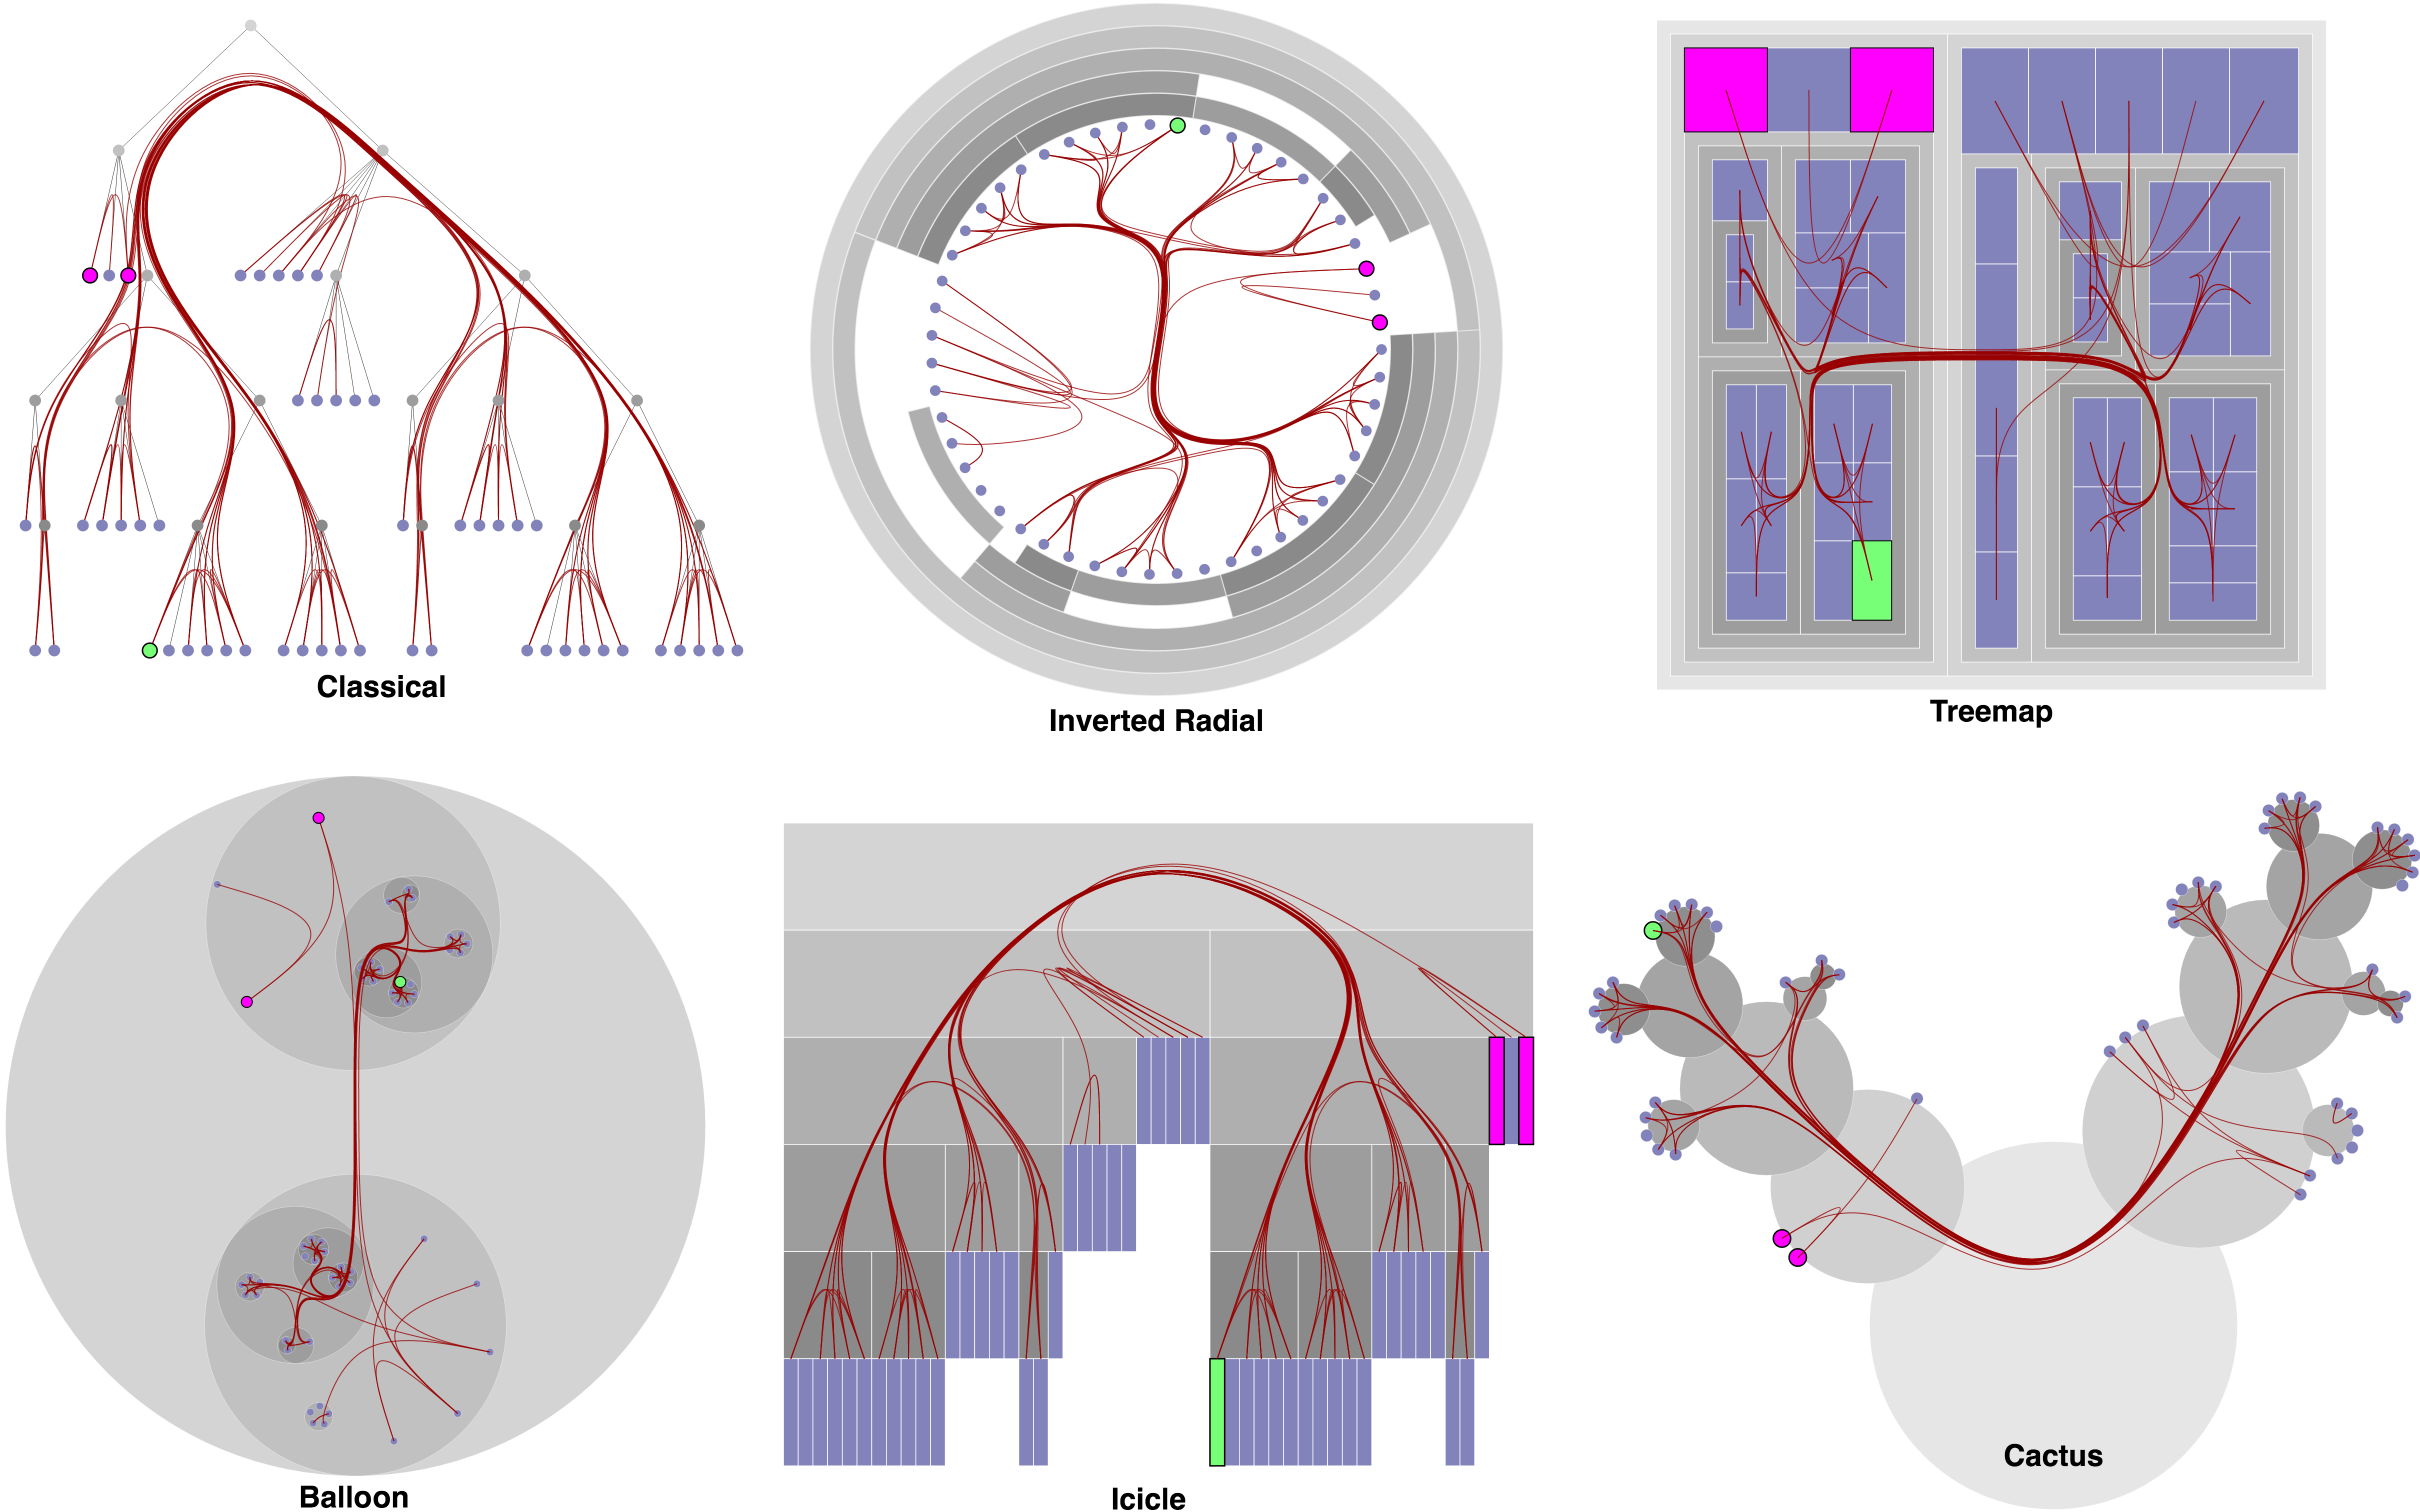
\includegraphics[width=\textwidth]{figures/Teaser.png}
 \caption{Examples of hierarchical edge bundling on a hierarchical dataset using different tree layouts. Connectedness between leaf nodes is more visible in some layouts than others: The two purple nodes are connected (via red links) and these purple nodes are disconnected from the green node.}
 \label{fig:teaser}
\end{figure}

\begin{comment}
	


\teaser{
   \centering
   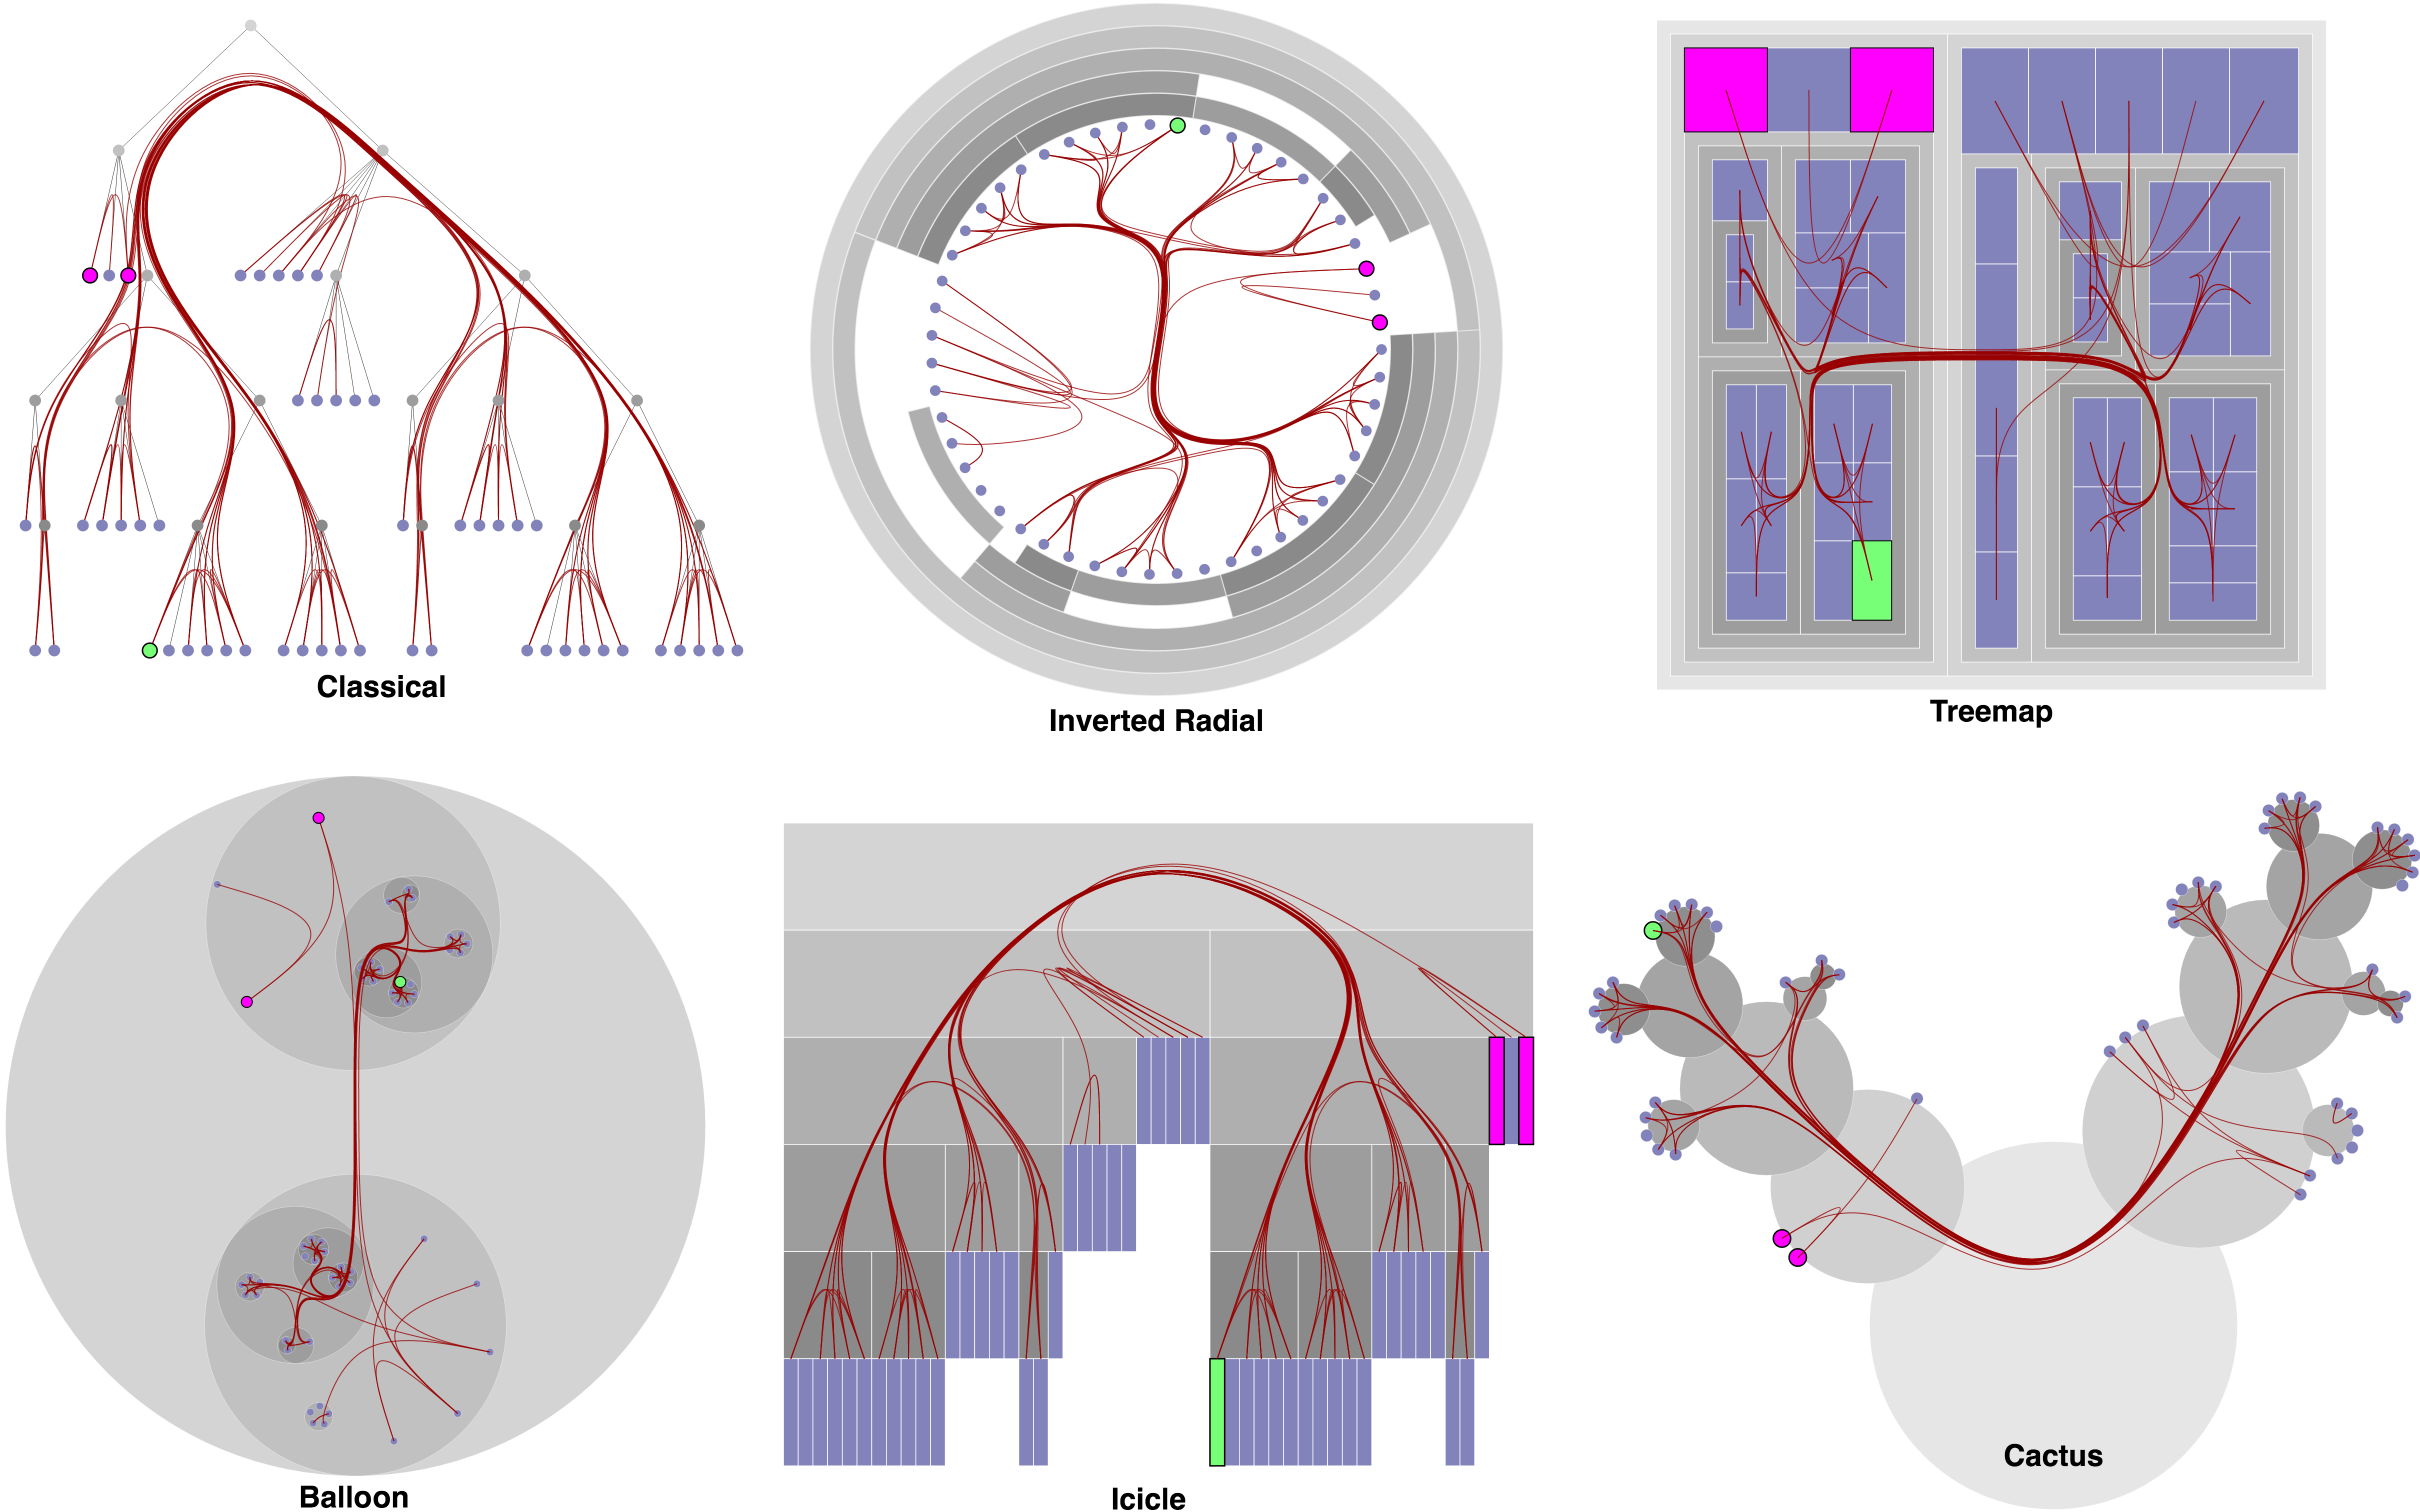
\includegraphics[width=\linewidth]{figures/Teaser.png}
  \caption{
  Examples of hierarchical edge bundling on a hierarchical dataset using different tree layouts. Connectedness between leaf nodes is better visible in some layouts than the others: The two purple nodes are connected (via red links) and these purple nodes are disconnected from the green node. %We leave it to the readers to select their choices of preference in this task.
  }
  \label{fig:teaser}
}

\end{comment}


\section{Related Work}

%This paper introduces a new tree visualization technique with the specific goal of untangling overlaid bundles of intersecting edges. That is, we aim to address the problem of collinearity, discussed in the original paper on hierarchical edge bundling~\cite{HierarchicalEdgeBundles2006}. Here, we discuss relevant work related to tree visualization and edge bundling.

%\subsection{Tree Visualization Techniques}

%A wide range of tree layouts have been introduced as general techniques to encode hierarchical data and in support of specific tasks.
Schulz~\cite{TreeVisSchulz} maintains \textit{Treevis.net}, a comprehensive website that describes of a large number of tree layouts (296 in total as of September 2017) gathered from conference proceedings and journal articles. Each of these layouts have advantages and disadvantages when used for particular tasks.
In this section, rather than attempting to survey all related visualization techniques, we instead highlight related work representative of the main approaches to visualize hierarchical datasets.

A TreeMap~\cite{shneiderman1992tree} is a space-filling technique that maps a hierarchical dataset onto a rectangular region. The effective use of space enables comparison of attributes of leaf nodes such as size and color coding, and therefore helps to highlight patterns and outliers in large hierarchies. ArcTrees~\cite{Neumann2005ArcTrees} additionally overlay non-hierarchical links onto TreeMaps~\cite{fekete2003interactive}. Icicle Plots~\cite{Kruskal1983IciclePlots} encode hierarchical data by stacking child rectangles directly on top of parent nodes. This makes it easier to see the hierarchical structure, but also assigns valuable screen space in assigning large areas to intermediate nodes. When using Icicle Plots to represent dense datasets that contain a large number of leaf nodes, the leaf nodes can be pushed close together, making them hard to see. Viegas et al.~\cite{viegas2013google} propose a solution to better utilize the space in a circle packing algorithm by defining a new center point of each ``balloon.'' However, the hierarchical structure can be difficult to interpret for tree datasets with more than a few levels of depth. 

Kobsa~\cite{Kobsa2004UserExperiments} describes a study to compare several well-known information visualization systems for tree hierarchies in a between-subjects experiment. The study showed a significant difference in completion times and correctness between structure-related versus attribute-related tasks on various tree layouts. McGuffin and Robert~\cite{McGuffin2010Trees} present an in-depth survey of tree layouts that introduces a range of metrics to define the information density of different tree layouts. These metrics provide design guidelines for the use of layouts for certain tasks, such as maximizing space-efficiency and supporting labeling.


%Clever variations of TreeMaps, including MartketMap~\cite{Wattenberg1999TreeMaps} and Squarified TreeMaps~\cite{Bruls99squarifiedtreemaps}, ensure low aspect ratio rectangles (where most rectangles are nearly square) replacing the ``slice-and-dice'' method used in the original TreeMap layout.
%Cushion TreeMaps~\cite{VanWijk1999CushionTreemaps} add intuitive shading to help improve the perception of hierarchical structure. Arbitrary polygons~\cite{Balzer2005VoronoiTreemaps} and circular glyphs~\cite{MiriahMeyer2012ClockMap} can be used instead of rectangles to create more visually attractive and useful layouts. Despite their popularity, TreeMaps can be difficult to decipher in some situations, such as when used to represent deeply nested hierarchies. 
%Beck et al.~\cite{beck2014generalized} introduce a generalization of Bosman's Pythagoras Trees to visualize arbitrarily branching hierarchical structures. Each node in the hierarchy is represented as a rectangle which is sized based on the collective size of its children. %Colors are used to encode the depth of nodes inside the hierarchy. This tree structure can also take a variety of forms that are created by adjusting different parameters such as length, width, order, and color. 
%While this technique has an appealing aesthetic quality, the gaps between areas representing hierarchical structure may interfere with how users perceive non-hierarchical connections between nodes. 



%%%%%%%%%%%%%%%%%%%%%%%%%%%%%%%%%%%%%%%%%%%%%%%%
 %For instance, to make it possible to ``bundle'' the edges without requiring a control mesh~\cite{cui2008geometryEB} or hierarchy, Holten and van Wijk~\cite{Holten2009ForceDirectedHEB} use a self-organizing algorithm. In this approach, edges are modeled as flexible springs that can attract each other while node positions remain fixed. Various factors, such as translucency~\cite{McGee2012StudyHEB}, color~\cite{Holten2009StudyHEB}, and depth effect, can be considered to aid in the perception of bundles. However, HEB is most often used as originally described~\cite{HierarchicalEdgeBundles2006}, and is readily available for some layouts via visualization toolkits, such as D3.js~\cite{bostock2011d3}.
%To the best of our knowledge, somewhat surprisingly,

%\subsection{Hierarchical Edge Bundling}
Hierarchical edge bundling (hereafter, HEB) groups links between adjacent edges by routing them through parent nodes in order to re-enforce the hierarchical structure of the data. HEB is widely used for a range of applications; however, HEB has not been evaluated systematically. In a survey paper on edge bundling techniques, Zhou et al.~\cite{zhou2013edge} summarize some studies of HEB, which tend to indicate user preference for visualizations that use HEB in comparison to those that do not. While not explicitly focused on HEB, Xu et al.~\cite{xu2012user} examine visualizations that use varying degrees of curvature, finding that links with high-curvature can adversely affect how well users interpret data. %Bach et al.~\cite{Bach2016confluentgraphs} investigate Confluent Drawings~\cite{Dickerson2004ConfluentDrawings}, a technique for bundling edges in node-link diagrams based on network connectivity. The authors also present a user study that compares edge-compression techniques, including Confluent Drawings, power graphs~\cite{Dwyer2013PowerGraphs}, ordered bundles~\cite{Pupyrev2012MetroStyles}, and edge bundling.
McGee and Dingliana~\cite{McGee2012StudyHEB} perform user experiments to evaluate the impact of bundling on user performance on different tasks using a set of randomly generated undirected compound graphs with varying sizes and edge densities. In their study, graphs are presented with a range of different levels of edge bundling using only a simple balloon tree layout. Moreover, the design of McGee and Dingliana's study limits the applicability of their results to 3 layers of depth and the interconnectivity in their generated graphs does not reflect real-world edge densities. %Finally, as we discuss below in Section~\ref{User Study}, the balloon tree layout--- the only layout they examined--- is not a good choice for HEB.

%Within the context of their experimental setup, their results indicate that bundling can actually hinder users in path tracing tasks, both in terms of accuracy and completion time. 

%Due to the lack of empirical data on the choice of tree representation for HEB, we conducted a user study to determine which tree layouts are more suitable for displaying complex compound graphs where HEB is used for highlighting non-hierarchical relations between data items. Ultimately, we want to derive design principles for effective visualizations of compound graphs.  







\section{Tree Qualities and Visualization Tasks}
\label{Sec:TheTasks}
There are many tasks related to visualizing compound graphs in a range of scientific domains, including those that involve biological pathways~\cite{Entourage2013}, ontology alignment~\cite{Nasir2013OntologyAlignment}, and taxonomic classifications~\cite{dang2015provenancematrix}. Although there are more basic tasks for tree layouts, such as determining the degree~\cite{Lee:2006TaskTaxonomy} or height~\cite{Wang:2006EvaluatingTree,Kobsa2004UserExperiments} of a tree, through in-depth discussions with systems biologists, taxonomists, and ontology researchers, we identified two primary tasks important for visual exploration of hierarchical datasets: characterizing hierarchical structures and identifying connections between nodes in the hierarchy.
%facilitate reasoning about connectivity.

%[Something about the specific tasks here... and how the following two tasks are necessary to support the more specific tasks... Like... downstream elements (using connections), or identifying redundant information (subtree), or being able to support visual comparison (subtree), etc. This will lead into T1 and T2...] 
%[]

%The biggest challenge in visualizing large hierarchical datasets is to mitigate their complexity, avoiding creating a ``hairball'' of links that are difficult to make sense of. When investigating large protein-protein interaction networks, for example, biologists are often interested in understanding causation. Causation in biological pathways can be understood as the downstream effects of any changes~\cite{beck2014state,Vehlow2016VisualizingDynamic}, for example, when a protein is perturbed as a result of drug treatment. Biologists need to better understand the complex structure of pathways, as well as to reason about the biochemical interconnection within and across multiple pathways. 

\noindent \textbf{T1: Effectively characterize hierarchical structure}---It is not uncommon find a pathway which contains more than ten nested levels~\cite{stromback2005representations}. Similarly, in taxonomic and ontological alignment domains, hierarchies can get extremely complicated, potentially containing thousands of leaf concepts~\cite{dang2015provenancematrix,TaxonomicProvenance2014}. More importantly, these classifications (hierarchies) can be contentious, and they may change from year to year as new discoveries or interpretations are made~\cite{Hinchliff2015phylogeny}. Having a representation which captures hierarchical structures effectively and allows users to visually identify structures/determine structural changes quickly is highly desirable by domain experts.

\noindent \textbf{T2: Minimize ambiguity introduced by edge bundling}---When HEB is applied, tracing a bundled link can lead to the perception of incorrect connectivity if edges are not clearly separated within the bundles~\cite{Bach2016confluentgraphs}. For some tree layouts the loss in detail (i.e., the ability to trace connectivity between two nodes) can be amplified depending on various factors, such as the chosen visual encodings and the overall structure of the tree. An ideal tree visualization technique to best support HEB should minimize this loss. 
 



\renewcommand{\arraystretch}{0.5}% Tighter
\begin{table*}[htb]
     \begin{center}
     \begin{tabular}{ l c c c c c c }
     \toprule
      &
  \raisebox{-\totalheight}{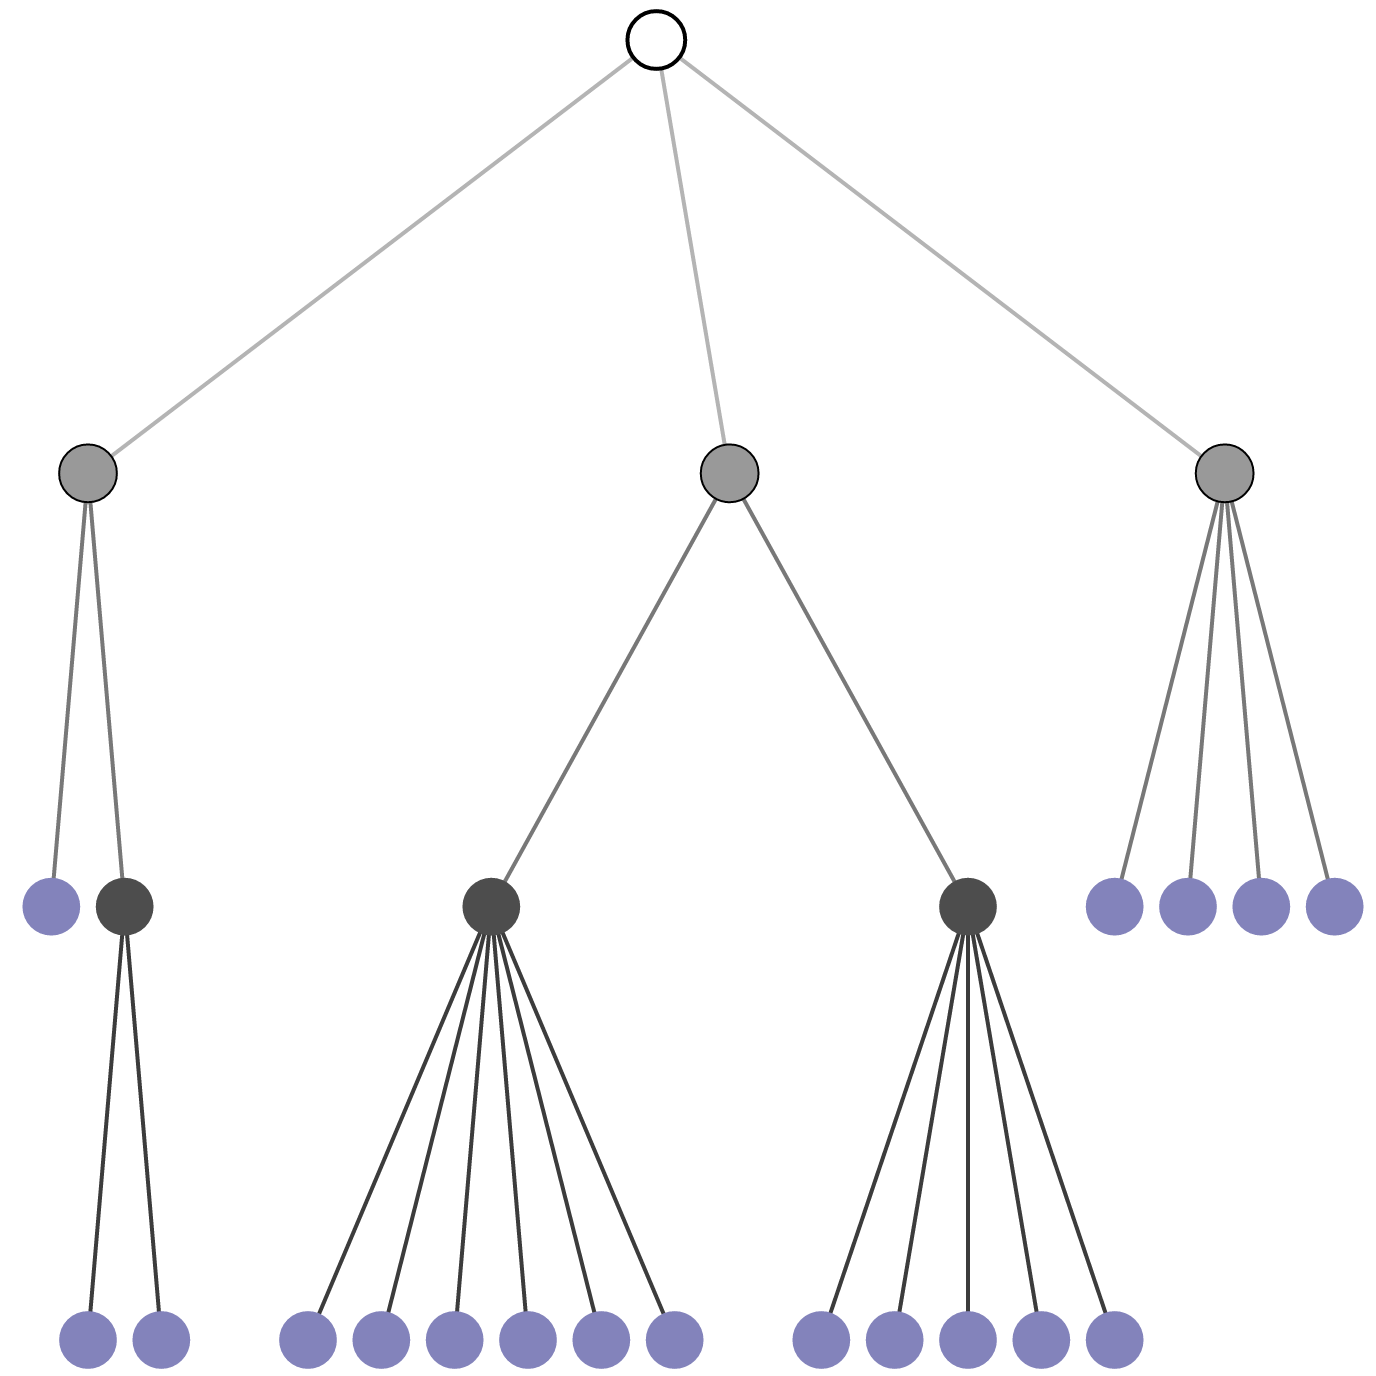
\includegraphics[width=0.111\textwidth]{figuresTable/TableClassical.png}}
      &
  \raisebox{-\totalheight}{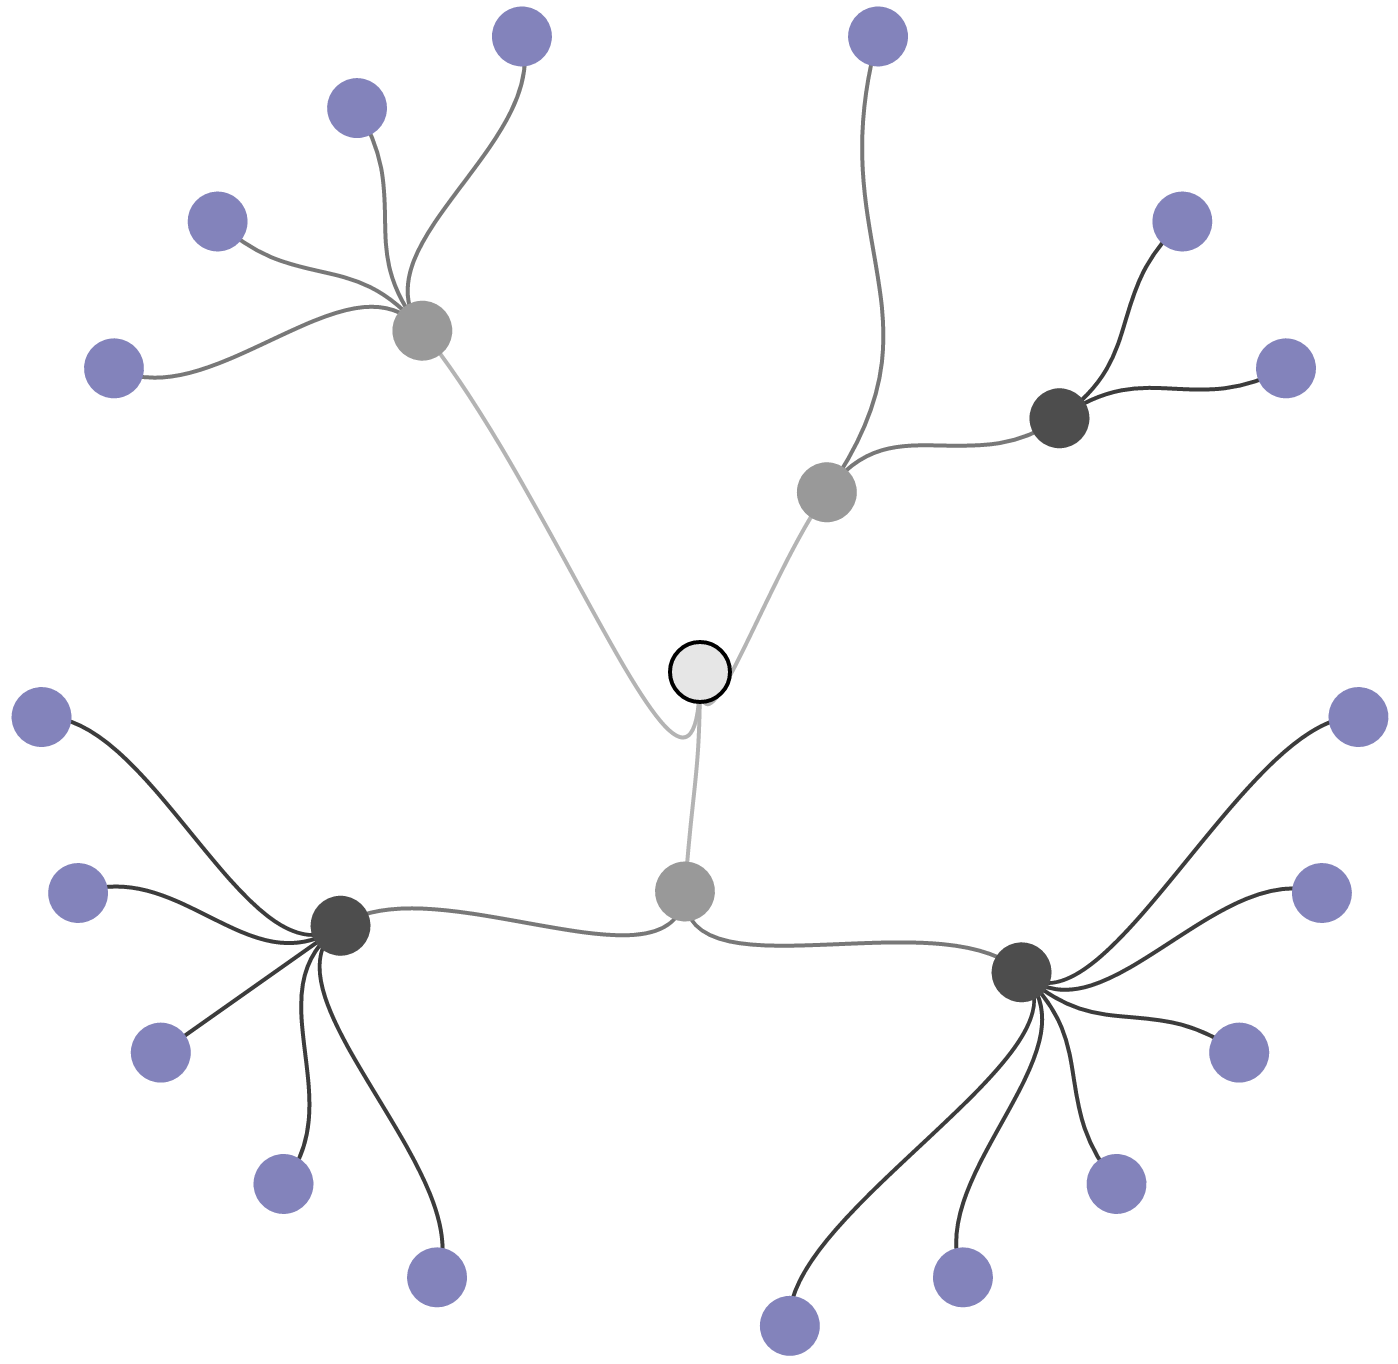
\includegraphics[width=0.111\textwidth]{figuresTable/TableRadial.png}}
      &
  \raisebox{-\totalheight}{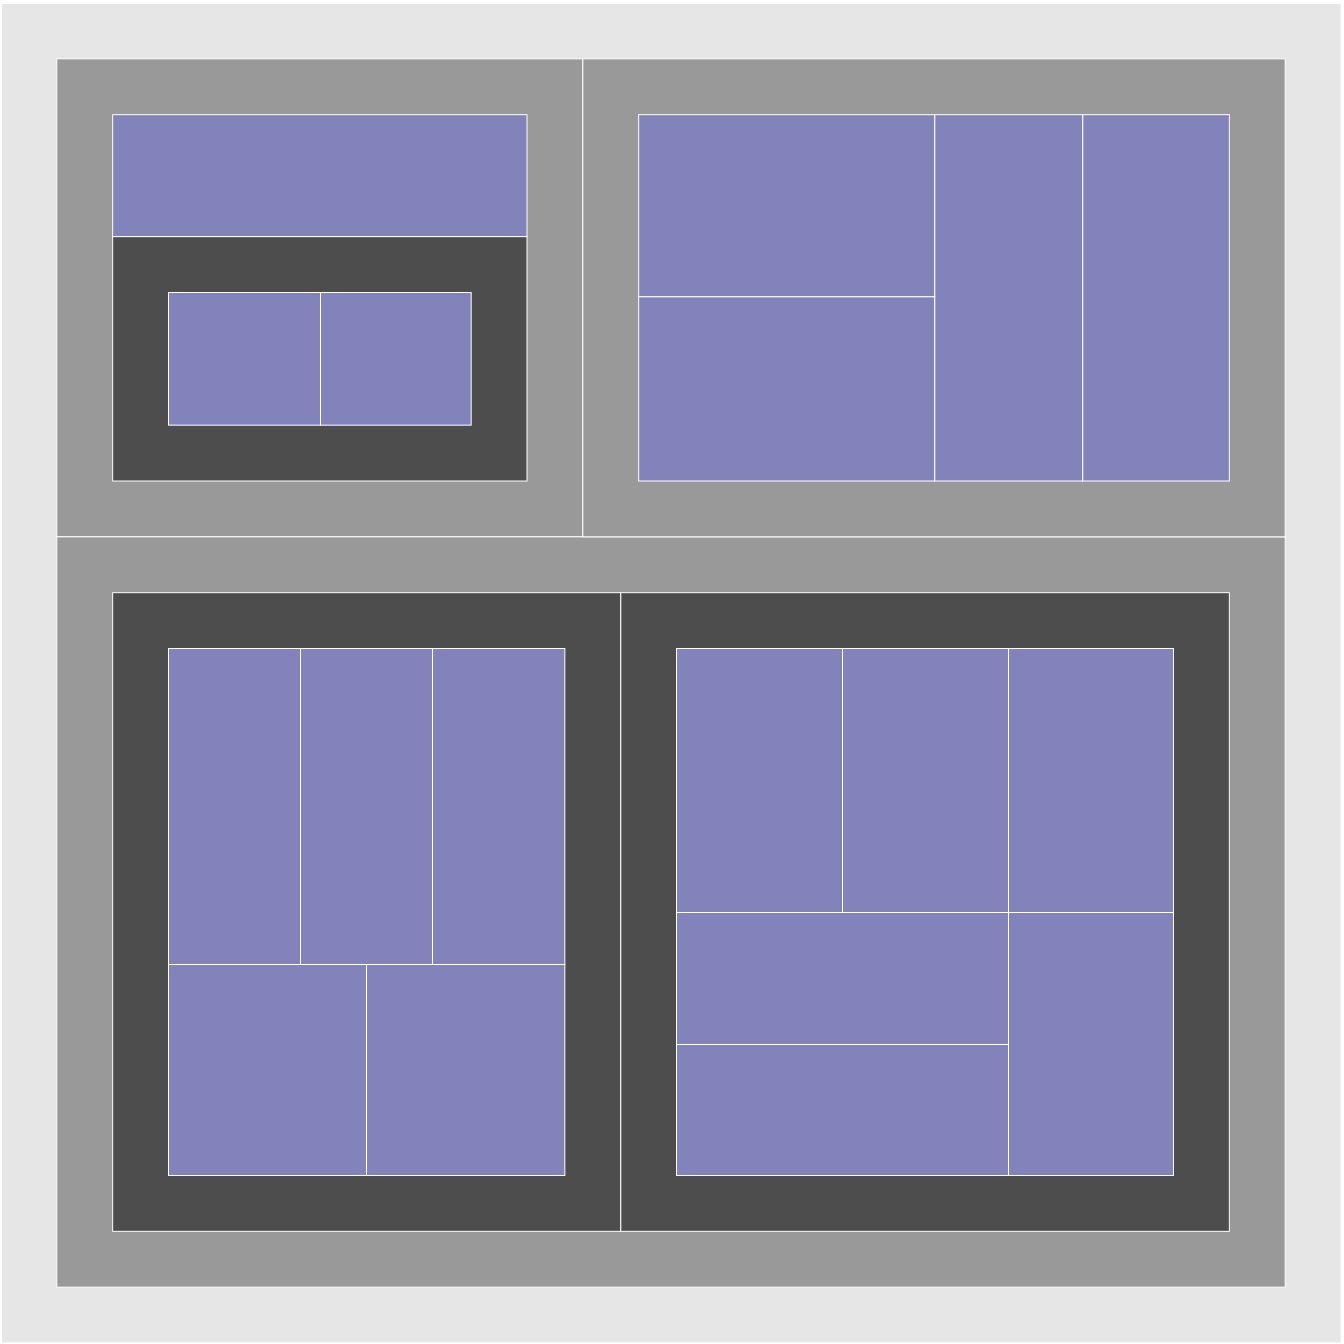
\includegraphics[width=0.111\textwidth]{figuresTable/TableTreemap.png}}
   &
  \raisebox{-\totalheight}{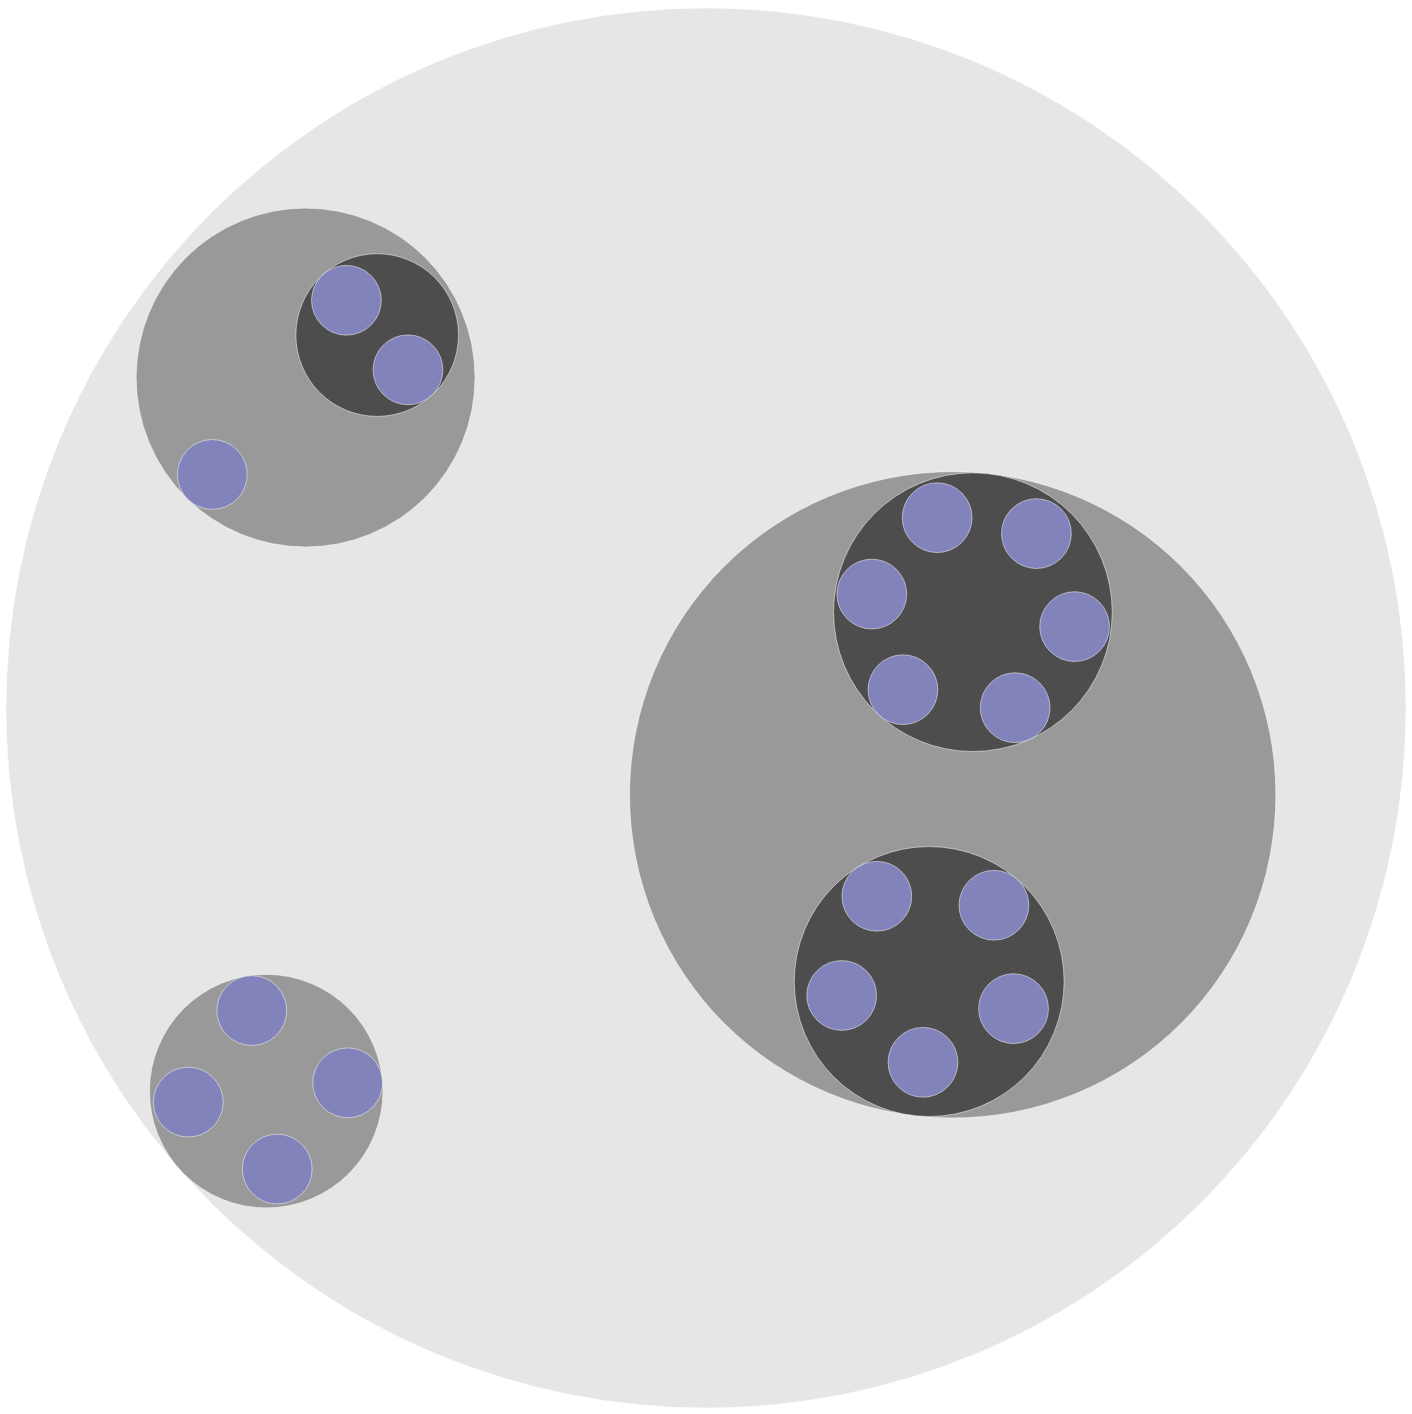
\includegraphics[width=0.111\textwidth]{figuresTable/TableBalloon.png}}
   &
  \raisebox{-\totalheight}{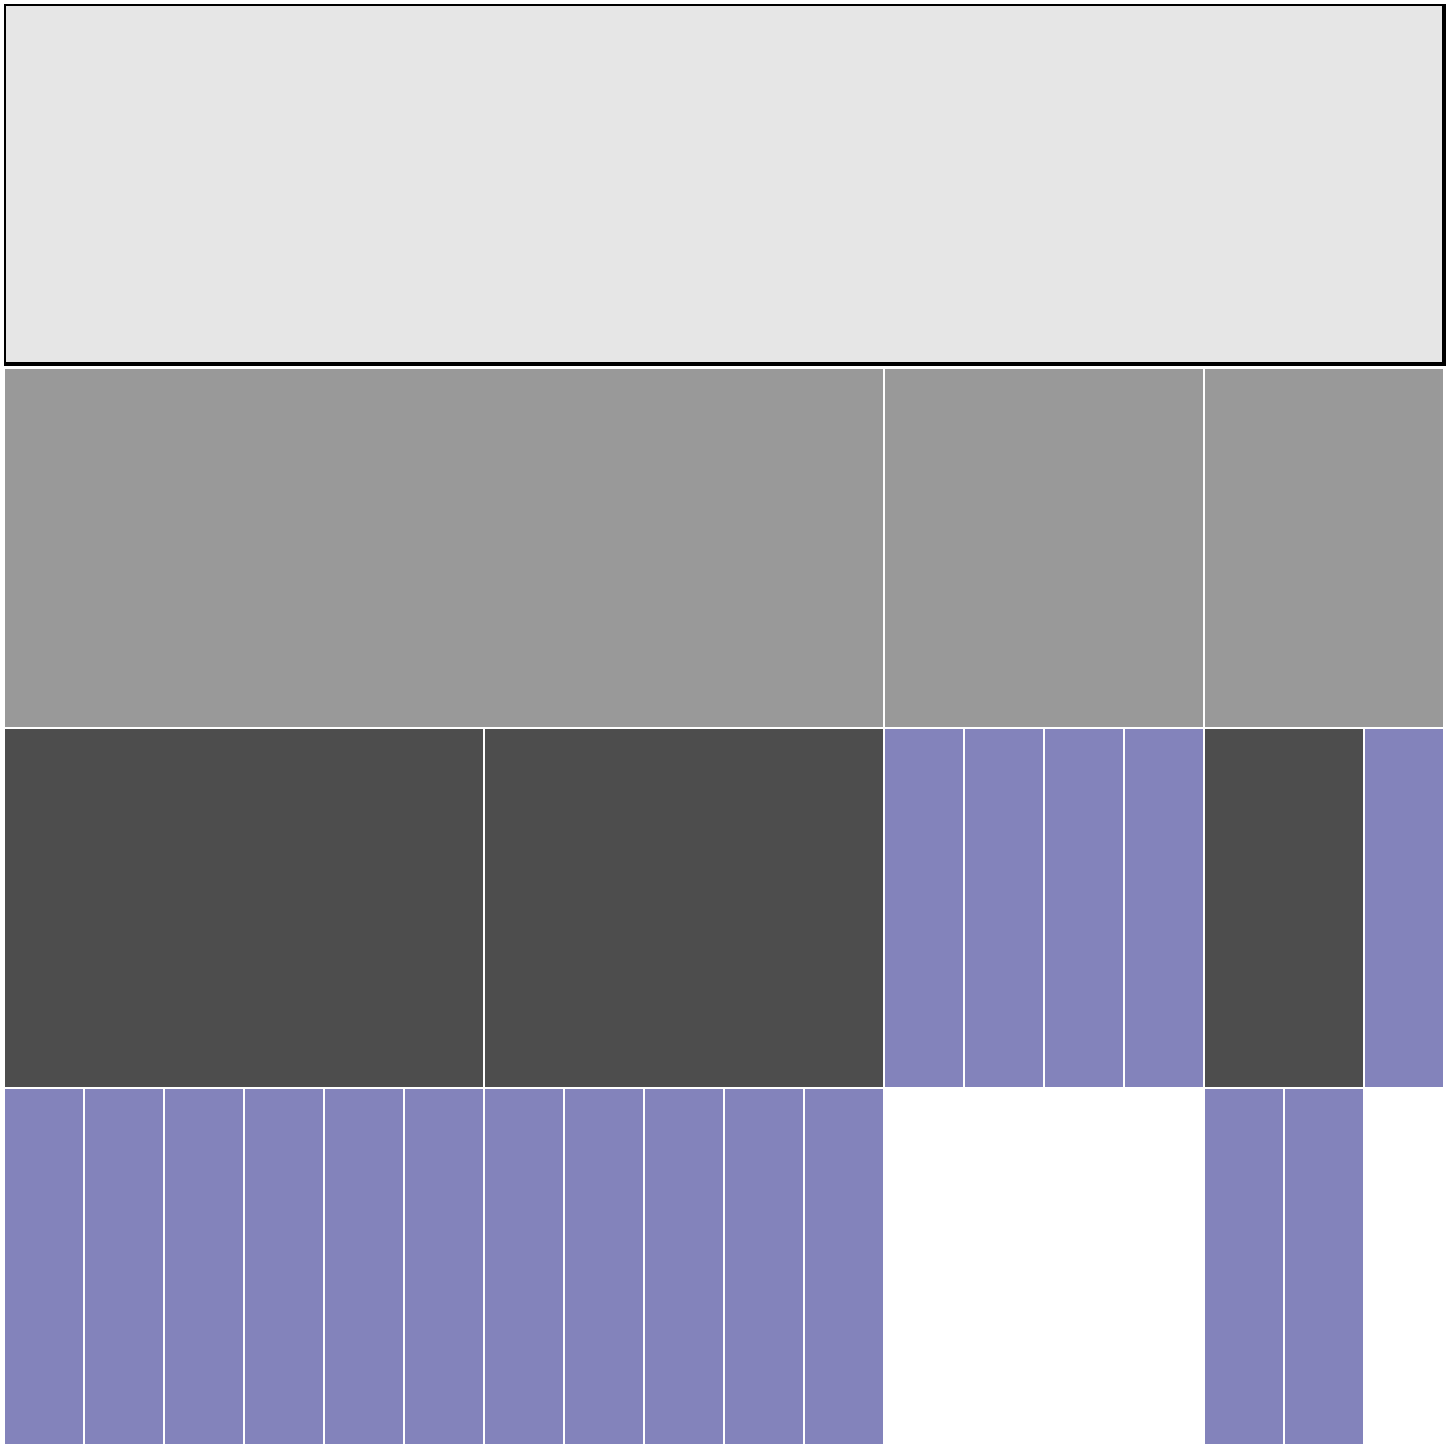
\includegraphics[width=0.111\textwidth]{figuresTable/TableIcicle.png}}
   &
  \raisebox{-\totalheight}{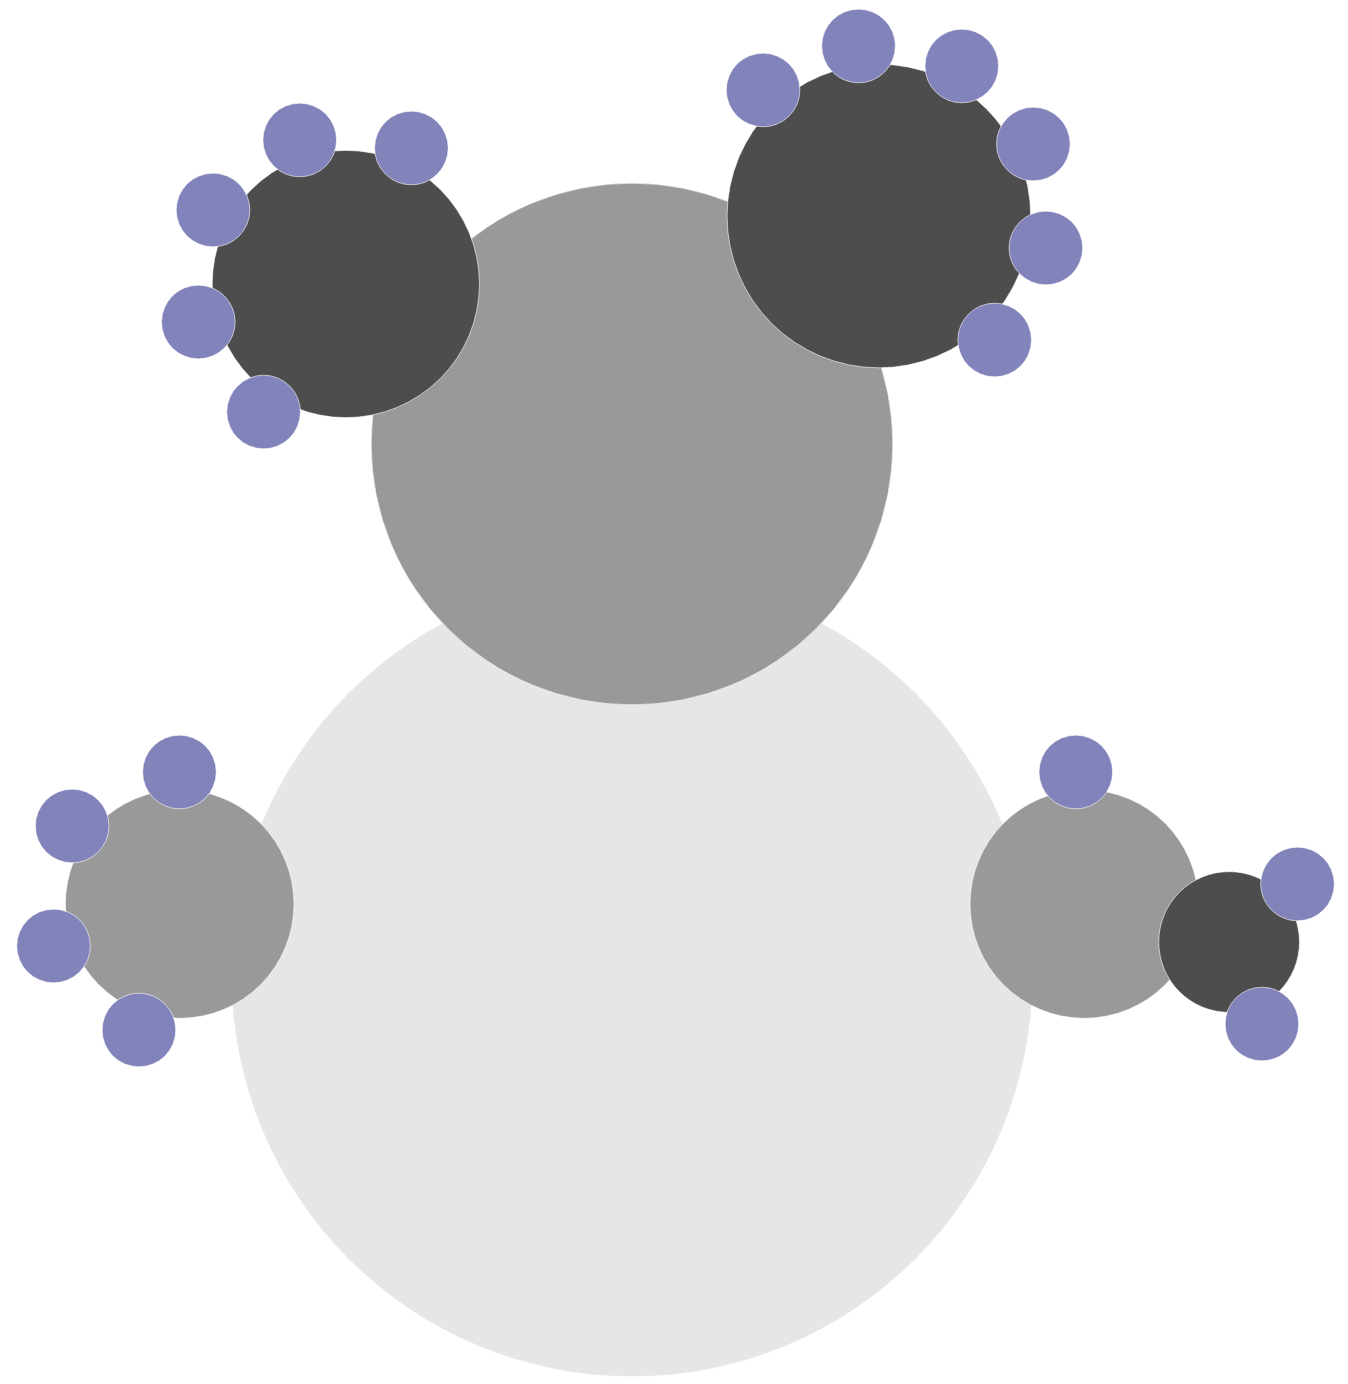
\includegraphics[width=0.111\textwidth]{figuresTable/TableCactus.png}}
  
    \\  
Tree layouts & Classic & Radial & TreeMap 
 & Balloon & Icicle & Cactus
 \\ 
   \cmidrule(lr){2-2}\cmidrule(l){3-3}\cmidrule(l){4-4}\cmidrule(l){5-5}\cmidrule(l){6-6}\cmidrule(l){7-7}
   Hierarchical relationship
\\ 
 ~~~~~Node-link &  \cellcolor{red!25}\checkmark  & \cellcolor{red!25}\checkmark  &  &  &  
\\ 
 ~~~~~Containment &    &   & \cellcolor{yellow!25}\checkmark & \cellcolor{yellow!25}\checkmark &  
\\ 
 ~~~~~Stacking & & & & & \cellcolor{green!25}\checkmark & \cellcolor{green!25}\checkmark
\\     
%\small{Node Alignment}
%\\ 
% ~~~~~\small{Axis-parallel} &  \checkmark  &   & \checkmark &  &  \checkmark   &
%\\ 
% ~~~~~\small{Radial} &    & \checkmark  &   & \checkmark &  &  \checkmark
%\\ 
Shape Preservation
\\ 
 ~~~~~Stable &  \cellcolor{green!25}\checkmark  & &  & \cellcolor{green!25}\checkmark & \cellcolor{green!25}\checkmark &  \cellcolor{green!25}\checkmark 
\\ 
 ~~~~~Malleable &  & \cellcolor{red!25}\checkmark & \cellcolor{red!25}\checkmark & &  & 
%\\ 
%Parent-child centers
%\\ 
% ~~~~~Non-overlapping & \cellcolor{green!25}\checkmark  & \cellcolor{green!25}\checkmark  &  & \cellcolor{green!25}\checkmark & \cellcolor{green!25}\checkmark  & \cellcolor{green!25}\checkmark
%\\ 
% ~~~~~Overlapping & &  & \cellcolor{red!25}\checkmark  &  &  & 
 
\\ 
Space-centric filling
\\ 
 ~~~~~Root-centric&   
 \cellcolor{red!25}\checkmark & \cellcolor{red!25}\checkmark  &  &  & \cellcolor{red!25}\checkmark  & 
\\ 
 ~~~~~Parent centric &  &  & \cellcolor{green!25}\checkmark  & 
 \cellcolor{green!25}\checkmark &  &  
 \cellcolor{green!25}\checkmark
  
\\ 
Bundling angularity
\\ 
 ~~~~~Wide &  &  &  & \cellcolor{green!25}\checkmark & & \cellcolor{green!25}\checkmark
\\ 
 ~~~~~Sharp & \cellcolor{red!25}\checkmark & 
 \cellcolor{yellow!25}\checkmark & \cellcolor{yellow!25}\checkmark & & 
  \cellcolor{red!25}\checkmark 
 & 
 
    \\ \bottomrule
      \end{tabular}
            
      \caption{Tree layouts and their qualities. Cells are colors based on our hypotheses about whether or not these qualities support the primary tasks in our user study (in Section~\ref{User Study}): red means that this quality will not effectively support these tasks; green means that it will be supportive; and yellow means that it falls somewhere in between or is neutral. %Radial and TreeMap layouts are hypothesized as neutral, as their malleable shape preservation makes this unpredictable on bundling angularity.
      }
      \label{table: tree qualities}
      \end{center}
\end{table*}


\subsection{Classifying Layouts to Support Visualization Tasks}
\label{classifyLayouts}

Hierarchical edge bundling can be used in conjunction with existing tree visualization techniques (balloon layout and radial cluster tree are the two prominent examples), but each layout introduces certain drawbacks. When we explicitly draw the hierarchy underneath the relationships (in the case of classic tree layout or TreeMaps), the visualization becomes more cluttered and it is difficult to interpret the hierarchical information. When we separate the hierarchy and connectivity (in the case of using outer rings to depict hierarchy in radial tree), it becomes less intuitive because viewers need to interpret them independently.


%Schulz et al.~\cite{schulz2013generative} further propose a generic tree layout pipeline to produce both implicit and explicit tree layouts. In this paper, we focus on layouts that support our primary tasks when applied to complex, real-world datasets. We look only at 2D graphical representations of tree structures (3D tree layouts are less popular and evaluating 3D tree layouts would require a more extensive investigation of  interactions, such as rotating, panning, and zooming).  


%Although there are hundreds of 2D graphical representations of tree structures~\cite{TreeVisSchulz}, they can roughly classified into three different categories based on how they are constructed:
%\begin{itemize}
%\item Using a \textit{node-link} approach to represent hierarchy (typical examples are the classic and radial layouts);
%\item  Using \textit{containment} to represent hierarchy (typical examples are TreeMaps and nested circles);
%\item  Using \textit{stacking} (i.e., a spatial arrangement) to represent hierarchy (typical examples are icicle and concentric circles). Our proposed technique (\theName) belongs to this category. 
%\end{itemize}


Schulz~\cite{TreeVisSchulz} classifies tree layouts in terms of three main features, based on their structural layout: \textit{dimensionality} (2D or 3D), \textit{representation} (explicit or implicit), and \textit{alignment} (axis-parallel, radial, and free). We refine Schulz's \textit{representation} categorization by further dividing implicit representations into two sub-categories, \textit{containment} and \textit{stacking}, in addition to \textit{node-link} representations. These categories have distinct features which impact the visual characteristics of HEB. In addition to refining the structural classification of the tree layouts, we also identified how the layouts are either amenable to or inappropriate for edge bundling techniques. We can thus characterize each tree layout in terms of the following four ``qualities'' (see examples of tree layouts in Table~\ref{table: tree qualities}). We hypothesize that, in each case, having a particular quality is superior to not having it, at least in terms of supporting our two primary tasks. We test this explicitly in Section~\ref{User Study}.


\subsubsection*{Hierarchical relationship: Node-link vs. containment vs. stacking} This describes the encoding of a parent-child relationship by either: (a) drawing a link (\textit{node-link}, such as in Classic trees or Radial trees); (b) nesting children within the parent (\textit{containment}, such as TreeMaps or Balloon layouts); or (c) having a spatial area of the child abut its parent (\textit{stacking}, such as Icicle plots). 
%\paragraph*{Node Alignment: axis-parallel vs. radial manner}. This is the categorization from TreeVis.

%\paragraph*{Outwardly vs. Inwardly Nested} abc
\subsubsection*{Shape preservation: Stable vs. malleable structure} How a subtree appears is affected by the structure of the tree (such as the number of leaf nodes) and where it locates in the tree. \textit{Stable} structures may have different scales/rotations, but overall shapes are preserved. A layout with a \textit{malleable} structure means that the exact same subtree may appear very different when positioned in different trees, or in different places within the same tree.

%\subsubsection*{Parent-child centering: Non-overlapping vs. overlapping centers}\noindent This indicates whether or not the layout presents the possibility of overlapping a child center with any of its ancestor's centers. \textit{Overlapping} can adversely affect HEB since the non-hierarchical relationship between two nodes are wired though their least common ancestor. Having a \textit{non-overlapping} centering avoids this possibility.

%\begin{wrapfigure}{r}{0.5\textwidth}
% \centering
% 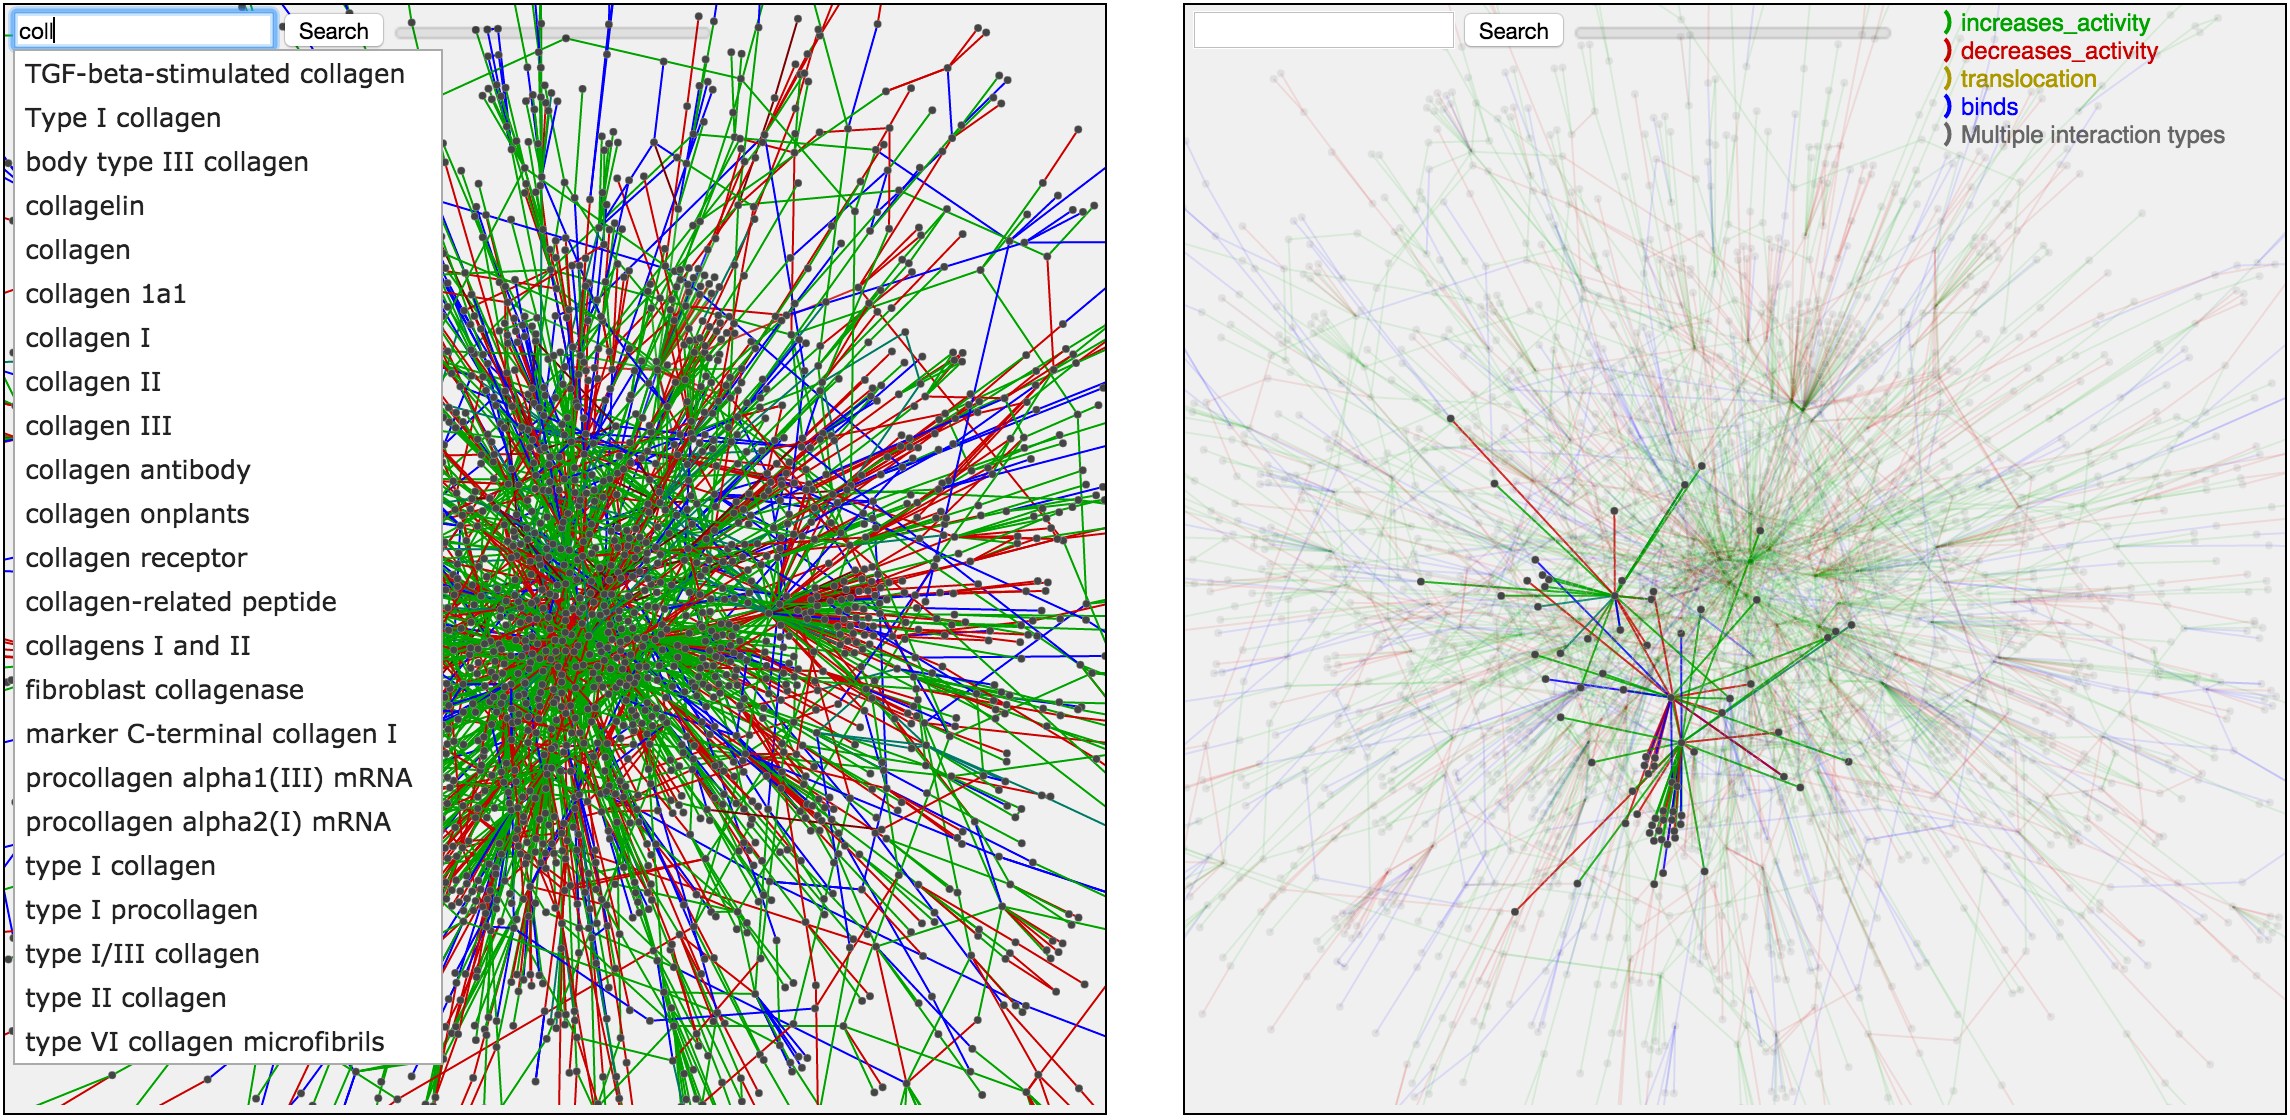
\includegraphics[width=0.5\textwidth]{figures/Figure2.png}
% \caption{\label{fig:Figure2} We hypothesize that bundled cross-edges in a \textit{parent-centric} layout (right) are more discernible than a \textit{root-centric} layout (left). Consequently, the \theName{} cell in Table~\ref{table: tree qualities} is colored in green while Icicle cell is colored in red w.r.t. space-centric filling quality. The hierarchy is the \textit{animate} subpackage structure within the  \textit{flare} software project. Each blue leaf node represents a source code file. Red links depict how these files refer each other.
 %}
 %\end{wrapfigure}
 
 
\subsubsection*{Space-centric filling: Root-centric vs. parent-centric} In \textit{root-centric} layouts, all layout operations are made with respect to the tree's root. In \textit{parent-centric} layouts, all layout operations are made with respect to a node's parent~\cite{schulz2013generative}. Based on this classification, Classic, Radial, and Icicle are \textit{root-centric} since the subdivision for leaf nodes are computed with respect to the root node. %Fig.~\ref{fig:Figure2} shows an example of \textit{root-centric} and \textit{parent-centric} layouts.% Icicle and \theName{} drawing strategies are very similar: child nodes are stacked directly on their parent nodes. However, the width of leaf nodes in Icicle plot (left) is equally divided based on root width, while child nodes in \theName{} are stacked along the half-arcs of their parent center with an assigned orientation (the \textit{alpha} input parameter in Algorithm~\ref{algorithm1}), and thus produces a \textit{parent-centric} layout. 
%The example in Fig.~\ref{fig:Figure2} gives an immediate impression of how the look and feel of the bundling changes when the layout is switched from \textit{root-centric} (Icicle) to \textit{parent-centric} (\theName{}). The hierarchical data in this example represents subpackages in the source code of the \textit{flare} software project.\footnote{http://flare.prefuse.org} 




\subsubsection*{Bundling angularity: Wide turns vs. sharp turns} This quality describes the ease of interpreting HEB overlaid on tree layouts. In general, layouts that have child nodes distributed in a linear manner with regard to their parent center have sharper turns than layouts that have child nodes distributed in a circular manner. For example, Radial trees (having child nodes distributed in a circular manner with regard to their root) have \textit{wider turns} compared to Classic trees and have \textit{sharper turns} compared to Balloon layouts (since Radial trees are \textit{root-centric} while Balloon layouts are \textit{parent-centric}). %Fig.~\ref{fig:Cactus1} provides examples that show the differences between sharp and wide turns. 
%In some cases, it is difficult to categorize a particular layout into \textit{sharp turns} or \textit{wide turns}, such as for layouts that do not preserve their shape (i.e., have a \textit{malleable} structure). For example, the bundling characteristics of a TreeMap depend on the relative position of child and parent nodes, which may be very different even between datasets that are quite similar. 




\section{User Study}
\label{User Study}
%\subsection{Participants and Apparatus}
For our controlled experiments we recruited 14 subjects (11 males and 3 females), aged between 22 and 38 with normal vision. All of the subjects had some familiarity with tree layouts, and a short training session was provided to give a further overview of each of the six layouts that were used in the study. The layouts shown to the subjects had sizes in the range 900x700 to 1200x1050 pixels. Subjects were allowed to touch the screen or to use a mouse or trackpad to move the mouse cursor, but the experiments involved no interaction (other than to select and confirm answers to the Yes/No questions).

The total length of the study (including two experiments) ran from between 30 minutes to just under one hour depending on the speed of the participant. The subjects were asked to answer the questions as quickly and accurately as possible. We collected accuracy and completion time for each quantitative task (described below); user preference data were also collected. The order of the questions was randomized to avoid bias and learning effects. 


%Within each category, we decided to select two typical tree representations to conduct the study. We end up with the final list of 6 trees which is consistent to McGuffin and Robert's survey~\cite{McGuffin2010Trees}.

%\subsection{Tree layouts}
For our user study, we chose representative examples of trees with the features described in Section~\ref{classifyLayouts}, including hierarchical relationship, shape preservation, space-centric filling, and bundling angularity. The 6 trees we used are shown in Table~\ref{table: tree qualities}: Classic, Radial, TreeMap, Balloon, Icicle, and Cactus. 

There are many variants of the same tree layout and multiple ways to visual encode them. Through a preliminary pilot study, we identified the best variant and visual encoding in each layout based on user performances. For example, for our representation of TreeMap, we decided to use a TreeMap with margins to better represent hierarchical structures. We also use gray shadings for all 6 tree layouts to encode different levels in the hierarchy; although some layouts may benefit from this encoding more than others. Examples of the layouts and their relevant features are presented in the top row of Table~\ref{table: tree qualities}, along with an indication of how well we thought the layouts would perform in our user study.

\subsection{Experiment 1: Identifying Subtrees}

 Our first experiment evaluates the ability of participants to identify the existence of a subtree within a larger tree. This task has been confirmed to be valuable by the domain experts we worked with to develop \textit{CactusTree}~\cite{Dang2017CactusTrees} and previous visualization techniques for representing interconnected hierarchical datasets~\cite{Dang2016_EuroVA,dang2015provenancematrix,Dang2015ReactionFlow,Dang2017_BioLinker_IEEEPacificVis,Dang2016a_IEEEEuroVis,biovisDang1}. For example, the \textit{RAF cascade} pathway (used in Table~\ref{table: tree qualities}, where it looks like a snowman in \theName{} representation) is duplicated four times in the larger \textit{Signalling by NGF} pathway.\footnote{http://www.reactome.org/PathwayBrowser/\#/R-HSA-166520} %(\theName{} is the rightmost layout in Fig.~\ref{fig:teaser}). 
In general, it can be important to facilitate hierarchical structure recognition tasks within tree layouts. For instance, in taxonomic studies, these taxonomic classifications may change from year to year (or even more often) as new discoveries are made~\cite{Hinchliff2015phylogeny}.


%\begin{wrapfigure}{r}{0.5\textwidth}
 %\centering
% 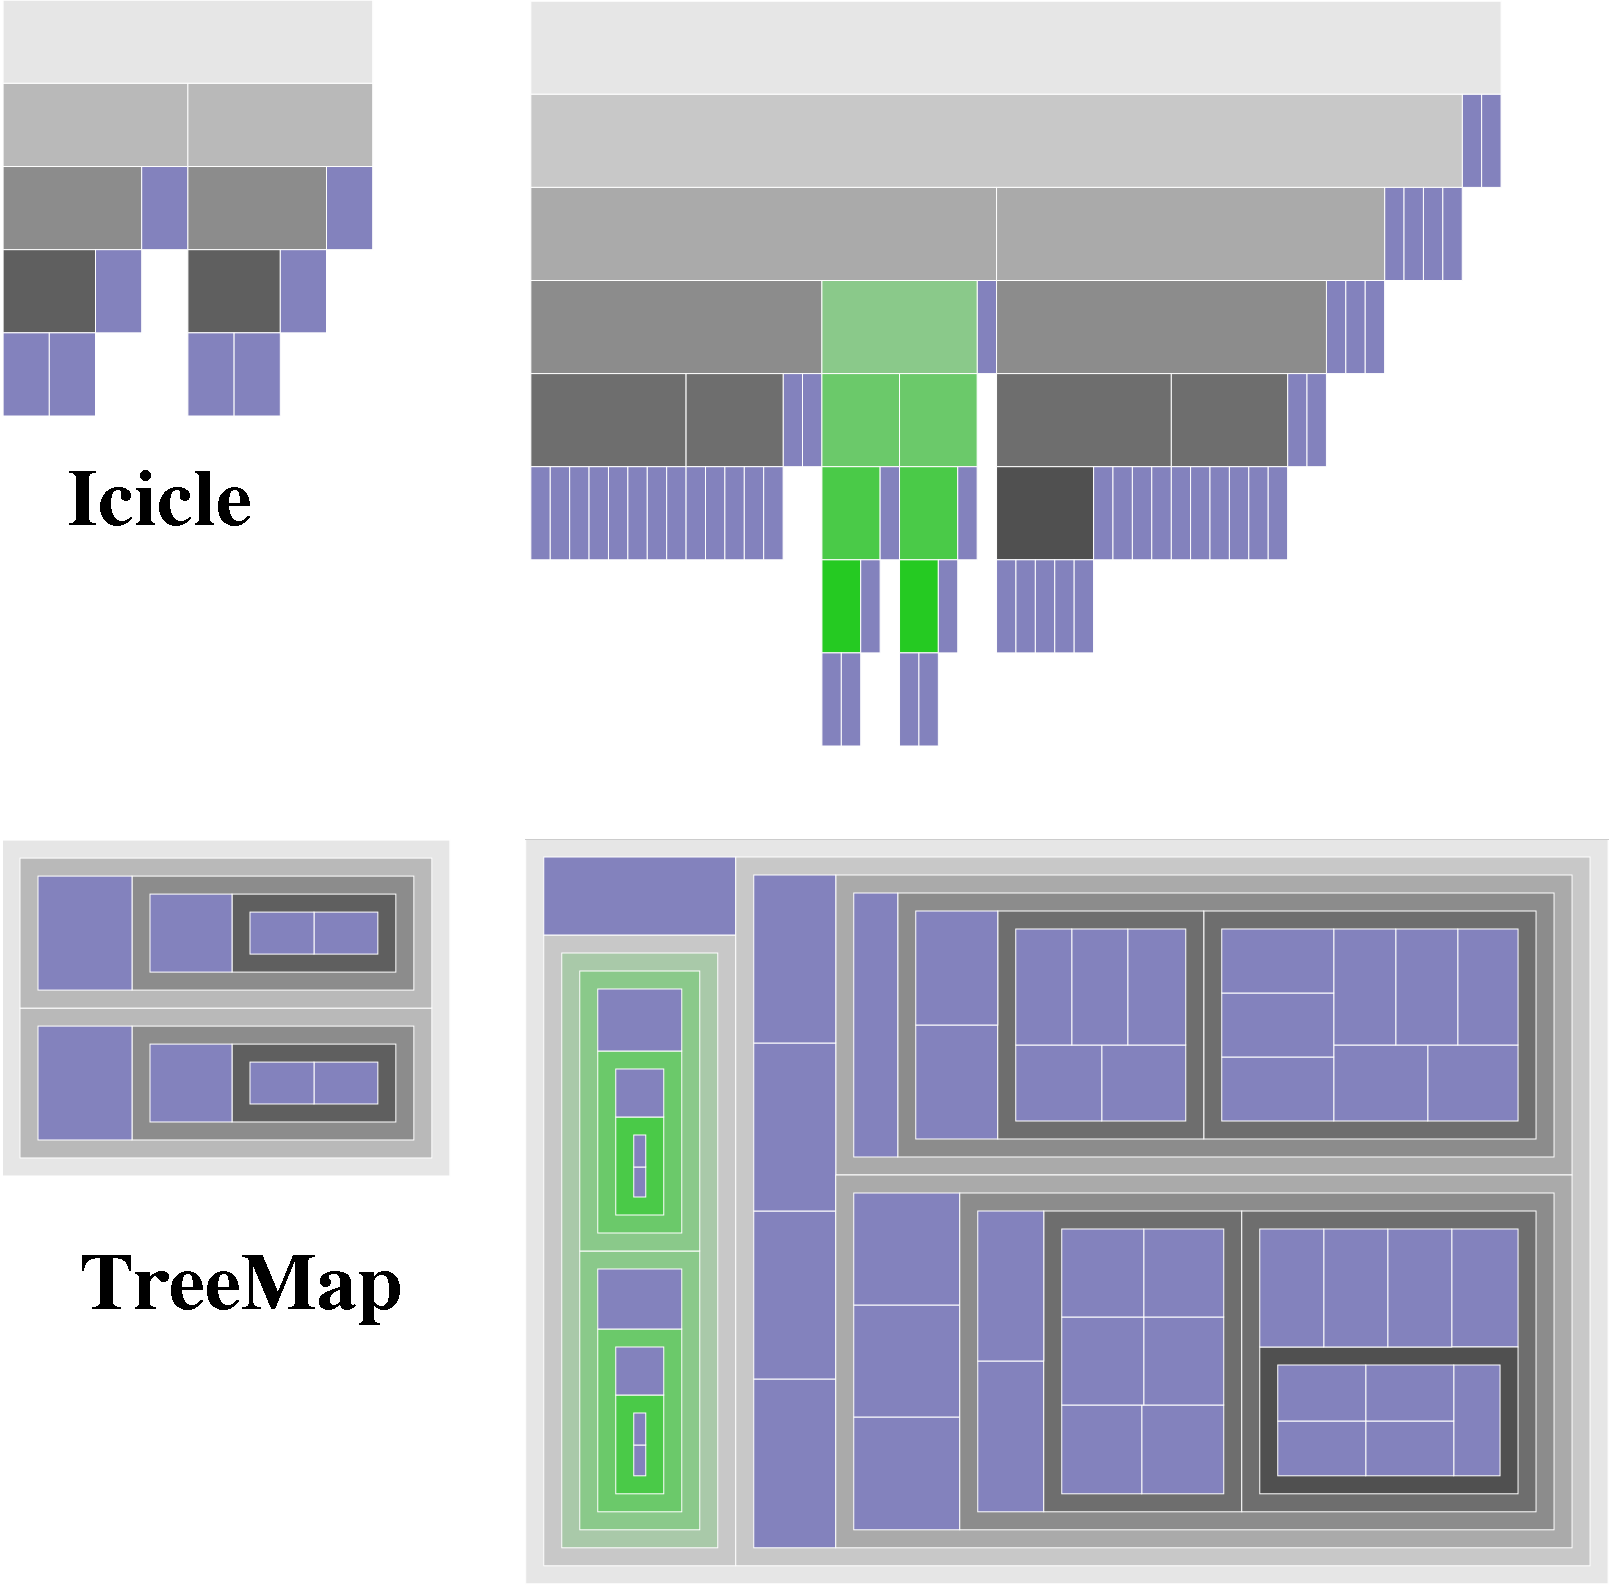
\includegraphics[width=0.5\textwidth]{figures/SubtreeExamples.png}
% \caption{\label{fig:SubtreeExamples} Examples of task 1 in Icicle and TreeMap on the same data. In each layout, the subtree is on the left, the larger search tree is on the right. Users are asked to identify if the exact subtree exists in the search tree. In this case, the answer is ``yes'' and highlighted in green.}
%\end{wrapfigure}
%Fig.~\ref{fig:SubtreeExamples} shows examples of the same data using Icicle Plot and TreeMap. In each layout, the subtree is on the left and the larger search tree is on the right. Users are asked to identify if the subtree exists in the search tree. In this case, the answer is ``yes'' and highlighted in green (but it is not highlighted in the actual study). Notice that for TreeMap the subtree appears very different as a standalone tree than within the larger tree, while for Icicle Plot the subtree more or less preserves its shape, only changing its scale and aspect ratio.


 
%\subsubsection{Experimental data}
In this experiment, we used 10 different datasets for subtrees, each of which were synthesized from real-world datasets from different domains, including biological pathways, \textit{flare} source code packages,\footnote{http://flare.prefuse.org} and mammal hierarchy~\cite{OneZoom2012}. We selected these datasets for subtrees because they characterize the inherent complexity of real-world scenarios. These subtrees have from 3 to 5 levels of depth. The depth of a tree is defined as the number of edges on the longest path from the root to a leaf. The degree of a tree is defined as the maximum degree of any of its nodes (the degree of a node is the number of its children).
The larger search trees are generated randomly with 6 level of depth and 6 degrees. Since our study does not explicitly evaluate zooming or other interaction techniques, these maximums ensure that the generated search trees are neither too small nor too large, which could cause a layout to be completely obvious or to draw tiny trees that are impossible for any user to recognize. %We also make sure that the randomized algorithm does not accidentally generate a search tree.

Our experiment was extended on the following dimensions: 6 tree visualizations x 10 subtree datasets = 60 questions. In particular, for each tree layout we asked 10 questions (associated with 10 subtrees) in which 5 contain a subtree and 5 do not. For those that do contain a subtree, we blend the subtree into a random position in the generated tree. The order of questions and tree layouts are completely randomized.
 %with in the first 3 levels (to make sure the search tree does not stand out at the leaf level even though this process may increase that search tree to 1 or 2 more levels of depth.  

\subsubsection{Hypotheses for the Identifying Subtrees Task} Based on our analysis of meaningful features for hierarchical structure recognition tasks, we hypothesized \textbf{H1}---Layouts that (a) preserve the shape of the data regardless of where it is positioned in the layout, and that (b) use \textit{stacking} to represent structure will perform better than those that do not, both in terms of completion time and accuracy, for the subtree task (\textbf{T1}). 

More specifically, we ranked the six layouts according to how these qualities were emphasized. Each tree layout exhibits these qualities to more or less of a degree, but generally, we expect shape preservation to be most important, followed by the type of hierarchical relationship. The following hypotheses about performance rankings are based on this expectation: \textbf{H1.1}---\textit{Cactus}, which can uniformly scale and rotate the shape, but do not otherwise modify it, will outperform all other layouts in terms of completion time and accuracy.
\noindent\textbf{H1.2}---\textit{Icicle}, which can narrow the nodes representing data when positioned within a larger tree, but otherwise retain its shape, will not perform as well as Cactus, but perform better than other layouts.
\noindent\textbf{H1.3}---\textit{Classic}, similarly to Icicle, can narrow the nodes representing data when they are positioned within a larger tree, and will not perform as well as Cactus. Classic will also not perform as well as Icicle since it also uses lines rather than shapes to indicate structure.
\noindent\textbf{H1.4}---\textit{Balloon}, although the shape of the data is preserved, nodes in general difficult to see because they are nested within each other, and become hard to view at deeper levels. Thus, Balloon will perform worse than Cactus, Icicle, and Classic, both in terms of accuracy and completion time.
\noindent\textbf{H1.5}---\textit{TreeMap} suffers from both having nested data and from lacking any guarantee that shape will be preserved. Thus, TreeMap will perform worse than Cactus, Icicle, Classic, and Balloon, both in terms of accuracy and completion time.
\noindent\textbf{H1.6}---\textit{Radial}, which does not preserve layout and uses lines to indicate structure, will perform worse than all other layouts, both in terms of accuracy and completion time.
 
 
 
\subsection{Experiment 2: Path Tracing}
Path tracing is a basic task in network visualization~\cite{McGee2012StudyHEB,Purchase1998Effects}. We asked participants to identify whether or not two highlighted nodes in a tree are connected using edge bundling. In our second experiment, we used 4 different datasets for subtrees drawn directly from real-world data used in different domains. The data was ranked in terms of its complexity, that is, its depth, number of leaf nodes, and number of links used in the edge bundling: \textit{easy} (4 levels, 3 max branches, 49 leaf nodes, 39 links); \textit{medium} (4 levels, 4 branches, 87 leaf nodes, 81 links); \textit{hard} (4 levels, 7 branshes, 105 leaf nodes, 156 links); and \textit{hardest} (4 levels, 7 branches, 103 leaf nodes, 267 links). We used these datasets because they reflect real-world, non-hierarchical link densities (the non-hierarchical links to the number of nodes). We further randomized these data by swapping 2 branches within 3 levels from the root. This generates more trees and ensures that participants will never see the same tree twice; swapping does not effect non-hierarchical link density. 

Our experiment was extended on the following dimensions: 6 tree visualizations x 4 datasets x 4 correct answers (2 Yes and 2 No)=  96 questions. Each pair of highlighted nodes was selected randomly. The order of questions and tree layouts are also completely randomized. The examples of the 4 original datasets in Cactus and Classic (without any blending or swapping of subtrees) are presented in Fig.~\ref{fig:Study2}, ordered from left to right in terms of difficulty of the increasing complexity of the data.

\begin{figure}[htb]
 \centering
 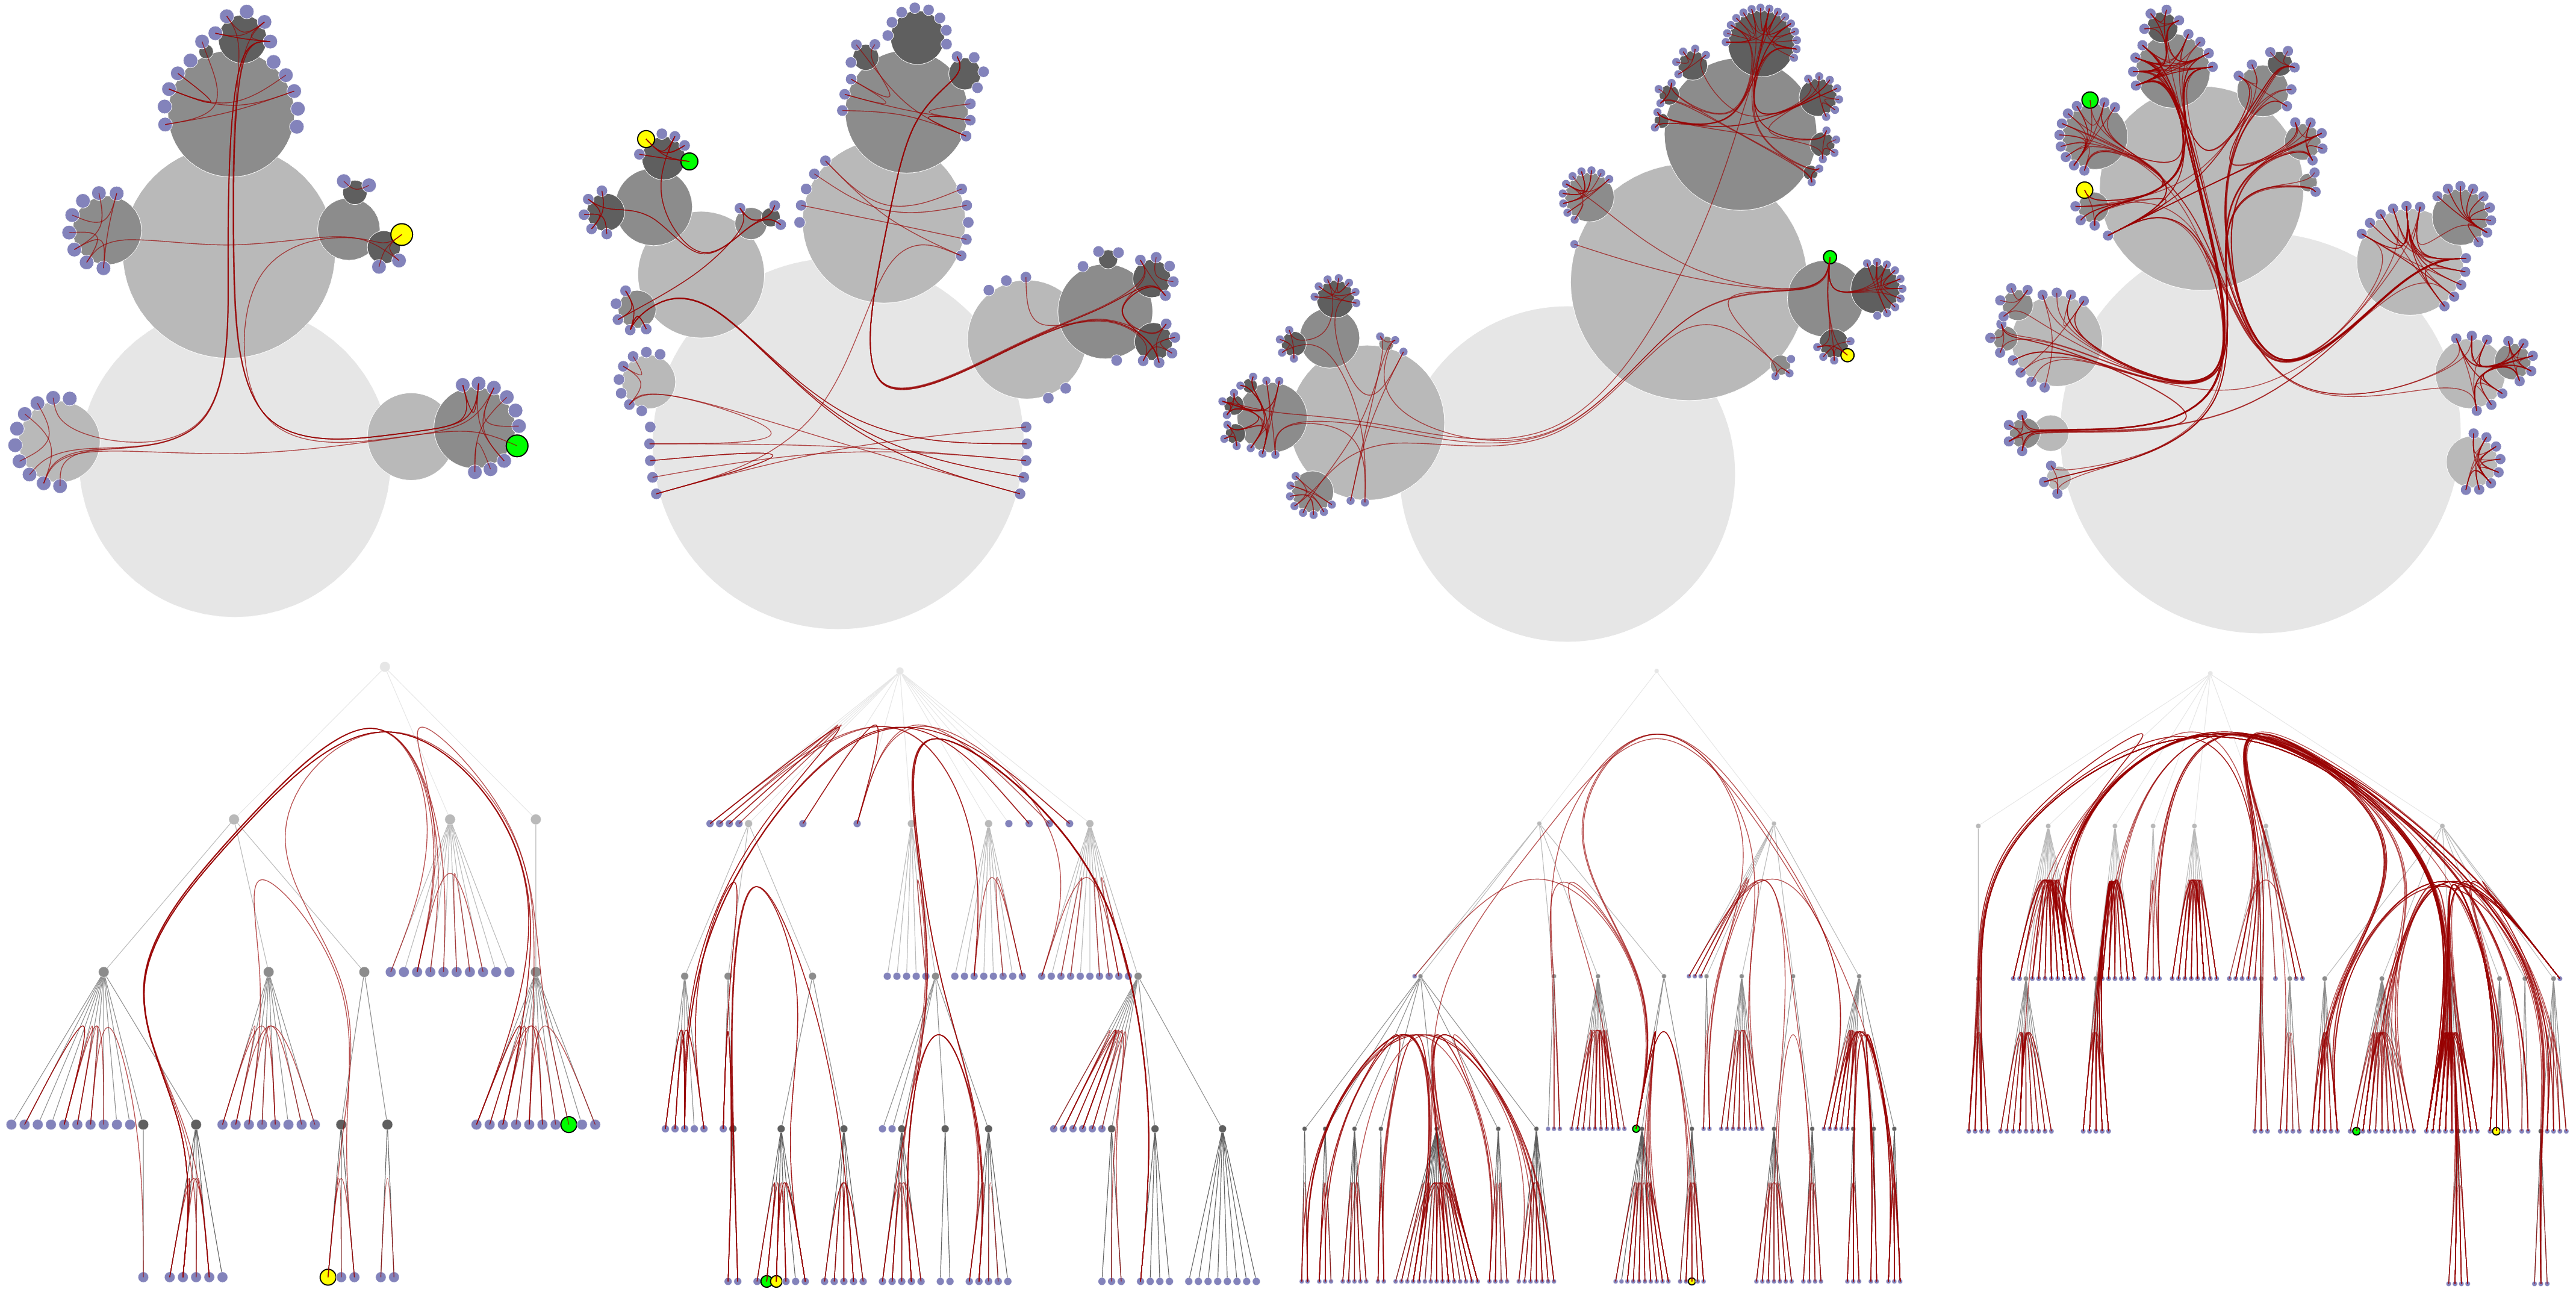
\includegraphics[width=\textwidth]{figures/Study2.png}
 \caption{\label{fig:Study2} Visualizing 4 input datasets using HEB on \theName{} (top row) and classic tree (bottom row). The difficulty of data increases from left to right. The same pair of nodes is highlighted in both tree representations for each of the four datasets.}
\end{figure}


\subsubsection{Hypotheses for the Path Tracing Task}
Based on our analysis of meaningful features for tree layouts, we hypothesized that layouts that emphasize a wider bundling angularity and that use a different visual encoding to differentiate hierarchical structure and non-hierarchical connectivity (i.e., containment and stacking) would perform better for the connectivity task: \textbf{H2}---Layouts that (a) use different visual encodings to represent hierarchy and connectivity, that (b) reduce sharp turns in edge bundling, that (c) and avoid inward nesting will perform better than those that do not, both in terms of completion time and accuracy, for the connectivity tracing task (\textbf{T2}). 

As with the first experiment, we ranked the six layouts according to how these qualities were emphasized. Each tree layout exhibits these qualities to more or less of a degree, but generally, we expect hierarchical relationship to be most important, followed by bundling angularity. The following hypotheses about performance rankings are based on this expectation: \textbf{H2.1}---\textit{Cactus}, which clearly differentiates between visual encodings and which uses a wide bundling angularity, will outperform all other layouts in terms of completion time and accuracy.
\noindent\textbf{H2.2}---\textit{Icicle}, which clearly differentiates between visual encodings but introduces sharp turns in edge bundling, will not perform as well as \theName{}, but will perform better than other layouts.
\noindent\textbf{H2.3}---\textit{Balloon}, which nests inwardly, but which supports wide bundling angularity  will perform worse than \theName{} and Icicle Plots in terms of both time and accuracy.
\noindent\textbf{H2.4}---\textit{TreeMap}, which nests inwardly, but uses a different visual encoding to differentiate hierarchical structure and non-hierarchical connectivity, will perform worse than Cactus, Icicle, and Balloon. 
\noindent\textbf{H2.5}---\textit{Radial}, which does not clearly differentiate between visual encodings, but which tends to have wider bundling angularity will perform worse than all layouts, except \textit{Classic} trees in terms of both time and accuracy.
\noindent\textbf{H2.6}---\textit{Classic}, which does not clearly differentiate between visual encodings, and which introduces sharp turns in edge bundling, will perform worse than all other layouts.


\section{Results}
Several aspects were considered for the statistical analysis of the results of the user study. First, we compared the six methods for each of the tasks by looking into the mean errors over all subjects and all data sets. Second, we did the same comparisons considering the time it took the participants to fulfill the tasks. For all analyses,\begin{wrapfigure}{r}{0.5\textwidth}
 \centering
 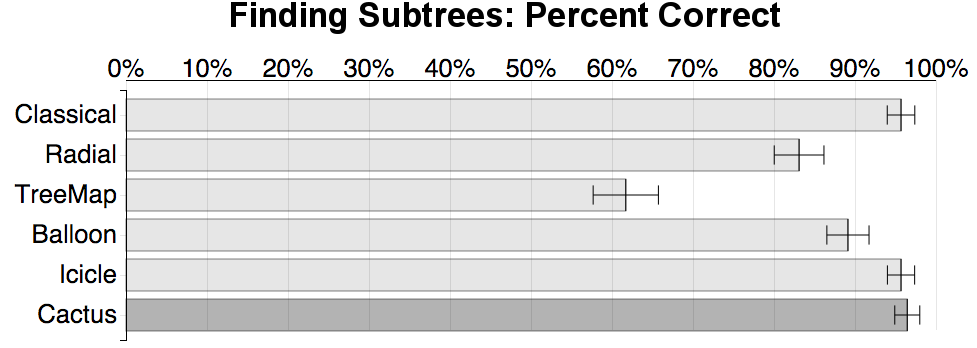
\includegraphics[width=0.5\textwidth]{figures2/T1-correct.png}
 \caption{\label{fig:T1-correct} Percent Correct (higher is better) for identifying subtrees (\textbf{T1}) for each of six layouts. Our \theName{} is highlighted in darker bars.}
\end{wrapfigure} we computed means and standard deviation of the errors. To test for statistical significance of the individual results, we first tested the distribution of the error values against normality using the Shapiro-Wilk tests~\cite{shapiro1965analysis}. All of our data had non-normal distribution, thus we applied the non-parametric Friedman test~\cite{friedman1937use} on K related samples when comparing more than two groups, and Kendall's Coefficient of Concordance~\cite{legendre2005species}. If the computed differences were significant, we performed pair-wise comparisons of the groups using a Wilcoxon test~\cite{wilcoxon1945individual} on non-parametric two related samples to be able to report which groups particularly differ from each other. For pair-wise comparisons in case of more than two groups we run a series of Holm's sequential Bonferroni adjustment at the 0.05 level. 
\subsection{Results of Experiment 1} Fig.~\ref{fig:T1-correct} summarizes the results of the comparative analysis of the six different methods for finding subtrees (\textbf{T1}). The bar charts show the mean error values and the standard error from the mean. The omnibus tests for statistical significance showed that there is statistical significance in the mean errors for some of the tasks. Kendall's Coefficient of Concordance test showed significant difference (Kendall W=0.149, $\chi^2$=102.76, df=5, p\textless0.01) among six methods. Bonferroni across pair-wise Wilcoxon comparisons showed significant differences between TreeMap and all other techniques, with TreeMap as the least accurate technique for finding sub-tree. Other pair-wise comparisons also showed significant differences: Icicle vs. Radial (Z=-3.343, P\textless0.0035), Cactus vs. Radial (Z=-3.34, P\textless0.0035) and Radial vs. Classic (Z=-2.942, P\textless0.0032). Therefore, according to Bonferroni adjustment, Icicle and Cactus are ranked as the best techniques. Classic is ranked as the second best technique. Balloon and Radial are ranked as the third best techniques and TreeMap is the worst technique.


%\begin{wrapfigure}{r}{0.5\textwidth}
% \centering
% 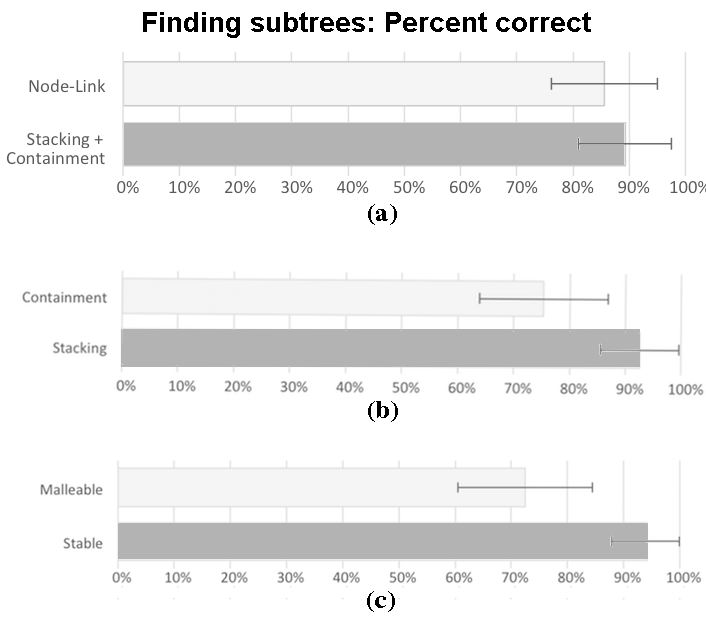
\includegraphics[width=0.5\textwidth]{figures2/T1-comparisons.png}
% \caption{\label{fig:T1-comparisons} Comparison of layout types on Percent Correct (higher is better) responses for finding subtrees (\textbf{T1}). Our \theName{} belongs to the group of darker bars.}
%\end{wrapfigure}
%For quality metrics, our statistical analysis showed a significant difference between the techniques that used either stacking or containment vs. node-link for hierarchical representation methods (Z=-2.967, P=0.003) and as shown in Fig.~\ref{fig:T1-comparisons}(a), they provide more accurate results significantly. Similarly, Wilcoxon signed-rank test showed a significant difference between the stacking representation and containment representation (Z=-6.835, P\textless0.0001), and, as shown in Fig.~\ref{fig:T1-comparisons}(b), they provide more accurate results. Additionally, a comparison between stable vs. malleable layouts shows a significant difference between them (Z=-6.114, P\textless0.0001). As demonstrated in Fig.~\ref{fig:T1-comparisons}(c), stable methods have a better performance for the subtree task.


Fig.~\ref{fig:T1-time} summarizes
the results of the time analysis of the six different methods for finding subtrees (\textbf{T1}). The bar charts show the mean error values and the standard error from the mean. The omnibus tests for statistical significance showed that there is
\begin{wrapfigure}{r}{0.5\textwidth}
 \centering
 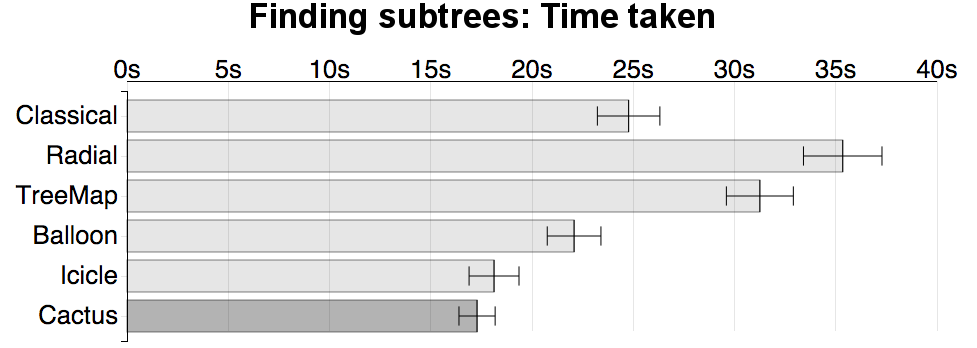
\includegraphics[width=0.5\textwidth]{figures2/T1-time.png}
 \caption{\label{fig:T1-time} Time taken (lower is better) for identifying subtrees (\textbf{T1}) for each of six layouts. Our \theName{} is highlighted in darker bars.}
\end{wrapfigure}
significance in the mean errors for some of the tasks. Kendall's Coefficient of Concordance test indicates significant difference (Kendall W=0.164, $\chi^2$=114.276, df=5, P\textless0.0001) among six methods. Pairwise comparisons between TreeMap and other techniques other than Radial Tree showed significant difference. TreeMap is one of the slowest techniques while Radial was significantly slower than TreeMap (Z=\mbox{-2.153}, P\textless0.031). Thus, Radial is ranked as the slowest techniques followed by TreeMap. The significant results from Bonferroni across pair-wise Wilcoxon comparisons between Cactus and Classic (Z={-3.747}, P\textless0.001) and Cactus and Balloon (Z=-2.986, P\textless0.003) also reveal Cactus to be one of the fastest techniques. Similarly, Icicle is ranked as one of the fastest method as revealed significant difference in comparison with Classic (Z=-4.178, P\textless0.001) and Balloon (Z=-2.548, P=0.011). These results show a consistent results with accuracy for finding because Icicle and Cactus both ranked as the two most accurate methods, while TreeMap was both the least accurate method and the slowest.



Thus \textbf{H1} is confirmed: layouts that use stacking to represent hierarchical structure are better than those that use containment or node-link representations; layouts that tend to preserve shape are better than those that do not. Our hypotheses about the importance of each of these qualities are mostly correct as well. Cactus and Icicle performed best (with no statistically significant difference), followed by Classic, then Balloon and Radial (which showed no statistically significant difference), and finally TreeMaps. Thus, \textbf{H1.1--H1.6} are partially supported. 




%%%%%%%%%%%%%%%%%%%%%%%%%%%%%%%%%%%%%%%%
\subsection{Results of Experiment 2}

Fig.~\ref{fig:T2-correct} summarizes the results of the comparative analysis of six different methods for path tracing tasks. Again, the bar charts show the mean error values and the standard error from the mean. The omnibus tests for statistical significance showed that there is statistical significance in the mean errors for some of the tasks. The Friedman test showed ($\chi^2$ (5,N=224)=3.250; P\textless0.001) among six methods. Bonferroni across pair-wise Wilcoxon comparisons showed significant differences between TreeMap vs. Cactus (Z=-3.255, P=0.001). Cactus outperforms significantly Icicle (Z=-4.096, P\textless0.0001). Cactus is also significantly more accurate than Balloon (Z=-4.216, P\textless0.001). Cactus is ranked as the best technique because it also has significantly better performance compared to Classic (Z=-2.263, P=0.024). Radial is ranked as the second best technique: TreeMap vs. Radial (Z=-2.967, P=0.003) showed significant difference. Radial vs. Balloon is also finds that Radial is significantly more accurate than Balloon. Classic ranked 
\begin{wrapfigure}{r}{0.5\textwidth}
 \centering
 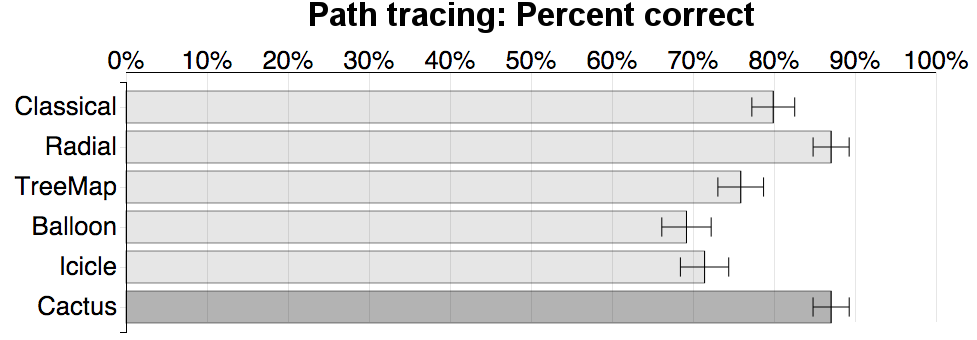
\includegraphics[width=0.5\textwidth]{figures2/T2-correct.png}
 \caption{\label{fig:T2-correct} Percent Correct (higher is better) for path tracing (\textbf{T2}) for each of six layouts. Our \theName{} is highlighted in darker bars.}
\end{wrapfigure}
third (Z=-2.449, P=0.014), while Balloon Layout, TreeMap, and Icicle are ranked as the worst techniques for \textbf{T2} regarding percent correct.

%\begin{wrapfigure}{r}{0.5\textwidth}
 %\centering
 %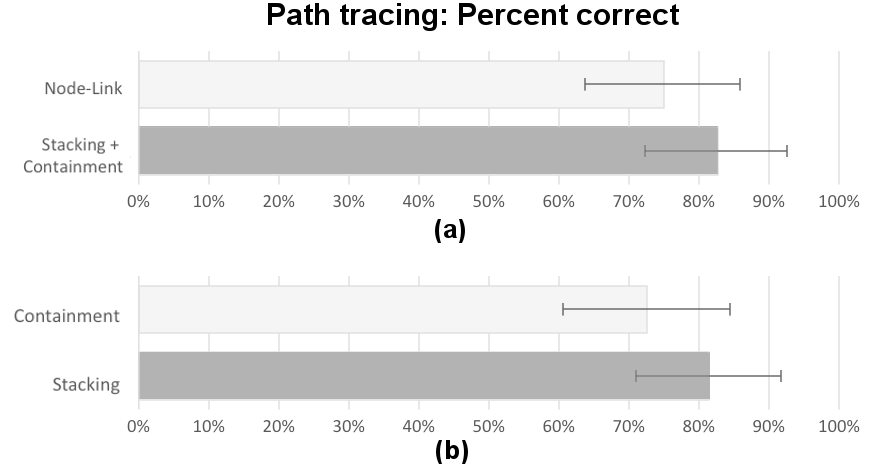
\includegraphics[width=0.5\textwidth]{figures2/T2-comparisons.png}
% \caption{\label{fig:T2-comparisons} Comparison of \textit{stacking} and \textit{node-link} layouts on percentage of correct responses (higher is better) for path tracing (\textbf{T2}). Our \theName{} belongs to the group of darker bars.}
%\end{wrapfigure}

%For quality metrics in Table~\ref{table: tree qualities}, our statistical analysis showed a significant difference between layouts that used a similar visual encoding for hierarchy and bundling vs. those that do not ($Z=-4.650,P<0.001$). As shown in Fig.~\ref{fig:T2-comparisons}(a), the stacking and containment layouts were significantly more accurate. Similarly, Wilcoxon signed-rank test showed a significant difference between stacking and containment techniques (Z=-2.188,P=0.029). Stacking techniques showed more accurate results as illustrated in Fig.~\ref{fig:T2-comparisons}(b).



\begin{wrapfigure}{r}{0.5\textwidth}
 \centering
 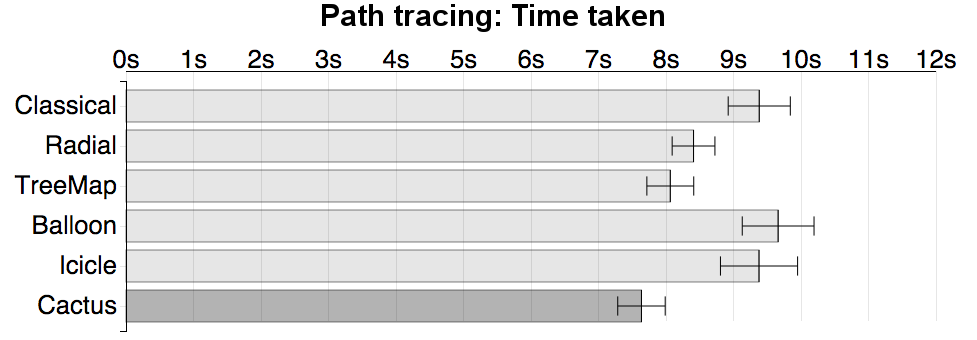
\includegraphics[width=0.5\textwidth]{figures2/T2-time.png}
 \caption{\label{fig:T2-time} Time taken (lower is better) for path tracing (\textbf{T2}) for each of six layouts. \theName{} is highlighted in darker bars.}
\end{wrapfigure}

Fig.~\ref{fig:T2-time} summarizes the results of the comparative analysis of the six different layouts in terms of the time taken to complete the path tracing task. The Friedman test showed significant difference ($\chi^2$ (5,N=192)=26.947; P\textless0.0001) among six methods. Pairwise comparisons showed significant differences between Cactus vs. Balloon (Z=-3.935,P\textless0.0001), Cactus vs. Classic (Z=-5.017,P\textless0.001), and Cactus vs. Icicle (Z=-2.849,P=0.004). However, based on Bonferroni adjustments, other pairwise comparisons did not reveal any significant results. We can therefore conclude that the \theName{} layout is significantly faster than all other methods for \textbf{T2}.


Thus \textbf{H2} is partially confirmed: layouts that use stacking to represent hierarchical structure are better than those that use containment or node-link representations. Our hypotheses about the ranking is only partially correct. Most notably, Cactus performs significantly better than all other layouts, in terms of both time and accuracy. %Thus \textbf{H2.1} is supported. 
However, our rankings of the others layouts was not as expected. In terms of accuracy, Radial performed second best, followed by Classic and Icicle, with no significant difference between them. The other two layouts performed poorly, with no significant difference between them. Thus, \textbf{H2.2}--\textbf{2.5} are not supported. Notably, Icicle was close to the bottom ranking, despite sharing many similar features as Cactus. We believe that this is largely due to the tendency of Icicle to introduce very narrow leaf nodes which are hard to distinguish from each other, especially when edge bundling is used to show connectivity between them.


We also compared the results of the Cactus, Icicle, and Radial layouts across the four different datasets, which had different levels of complexity, from C1 (simplest) to C4 (most complex). For Cactus, the Friedman test did not show any significant differences among all levels of complexities. That is, the Cactus layout performed equally well across all levels of complexity. However, the Friedman test showed significant differences among different levels of complexity for Icicle ($\chi^2$(3,N=56)=22.105; P\textless0.001). Wilcoxon pairwise comparisons showed significant differences between C3 vs. C1 (Z=-2.324, P<0.001), C3 vs. C2 (Z=-2.744, P=0.006), and C4 vs. C3 (Z=-3.530, P=0.001). That is, the accuracy of Icicle  tends to get worse as the data becomes more complex.
Similarly, the Friedman test showed a significant differences among different levels of complexity for Radial (($\chi^2$(3,N=56)=27.370; P\textless0.001). Wilcoxon pairwise comparisons showed significant differences between C3 vs. C1 (Z=-3.578, P\textless0.001), C3 vs. C2 (Z=-3.411, P=0.001), and C4 vs. C3 (Z=-3.273, P=0.001). As with Icicle, the accuracy of Radial tends to get worse as the data becomes more complex. The other layouts showed no significant differences between the different levels of complexity. 


\ \\ \

\renewcommand{\arraystretch}{1}% Tighter
\begin{table}[htb]
     \begin{center}
     \begin{tabular}{ l c c c c c c }
     \toprule
 
    & Classic & Radial & TreeMap 
 & Balloon & Icicle & Cactus
 \\ 
   \cmidrule(lr){2-2}\cmidrule(l){3-3}\cmidrule(l){4-4}\cmidrule(l){5-5}\cmidrule(l){6-6}\cmidrule(l){7-7}
   \textbf{T1} & 3 & 4 & 6 & 5 & 1 &1
\\     
    \textbf{T2} & 4 & 2 & 5 & 6 & 3 &1

    \\ \bottomrule
      \end{tabular}
            
      \caption{Average user preferences on different tree layouts for the two tasks: finding subtrees (\textbf{T1}) and path tracing (\textbf{T2}), 1 = best, 6 = worst. Icicle and Cactus are both the best for \textbf{T1}.}
      \label{table: tree rating}
      \end{center}
\end{table}


\subsection{Qualitative Responses}

In addition to recording the participants' time and accuracy of questions related to each of the tasks, we also solicited qualitative responses about each of the layouts. At the end of the study, each user was invited to rank the layouts and to offer comments. User preferences for the two tasks in our study in Section~\ref{User Study} are shown in Table~\ref{table: tree rating}.
    
Despite the general familiarity with the Classic tree layout by the participants, they had mixed responses to it. Some participants indicated that it was among the best techniques with which to identify subtrees, but others noted that it was hard to trace paths between nodes on the tree.  

    
    
    All participants mentioned that they liked the patterns created by the TreeMap layout, but most also indicated that it was frustrating to find structural patterns and that it was confusing to trace connections between the nodes using the TreeMap. This was especially when the links inadvertently crossed the center of a node, as it was hard to tell which level was being indicated. As one user noted, ``sometimes it seems as if the connections are connected through an intermediate step.'' One exception was a user who rated the TreeMap highly despite the visual clutter, saying that ``it just seemed easier to recognize connections, even when the data was messy.''
    
    Participants also mentioned that they were drawn to the Radial layout, but that, as one user said, ``if there were too many layers, it became very complicated to see if the subtrees were in there''--- A sentiment echoed by most users. On the other hand, the Radial layout was evaluated much more favorably for the path tracing task. The Balloon layout was perceived the most negatively by participants, as it was acknowledged by all participants that they were difficult to interpret for the more deeply nested trees. 
    
    CactusTree and Icicle Plots were described most positively by participants. They found both of these techniques to be more ``intuitive'' to understand, but some noted that it was harder to read the Icicle Plots in some cases when the density of the tree caused nodes to be narrow: ``It was hard to read the connections in the normal [Classic] tree, because the lines seemed stitched together, and the same thing happens with the Icicle tree.'' Participants were prone to find unintentional patterns in the CactusTree layout, noting that some trees looked, variously, like ``snowmen,'' ``clouds,'' ``animals,'' or ``a face.'' However, this didn't seem to present a distraction, as nearly all participants found it easy to identify subtree patterns in this layout and indicated that it was the most straightforward technique with which to trace paths between nodes. 
    
  



%\subsection{Discussion of Results}




\begin{comment}
\subsection{Task 1}
This task involving identifying subtrees in a larger tree. Duplicated subtrees exist among alternative taxonomies as confirmed by taxonomy experts. 

\textbf{H1}: Cactus will outperform all other layouts in completion time and accuracy for \textbf{T1} since it involves shape recognition. 

Icicle will outperform all other layouts except Cactus tree in accuracy and completion time.

Classic tree will outperform all other layouts except Cactus tree and Icicle plot in accuracy and completion time. 

Balloon layout is as good as Cactus tree in accuracy for smaller search tree but the nodes quickly become too small for larger search tree and so Balloon layout will underperform Cactus tree, Icicle plot, and classic tree in in accuracy and completion time. 

Radial tree will outperform TreeMaps in accuracy for the subtree task but will underperform other layouts completion time and accuracy since it requires time to count leaf nodes.

TreeMaps will underperform all other layouts in accuracy because it depends on how complex the search tree is and where the subtree appears in the search tree. 

\subsection{Task 2}
This task involving identifying if two leaf nodes are connected. This is the main task but we nee Task 1 because Task 2 depends on Task 1 (bundling algorithm works on the structure of a tree)  

H2.1: Cactus is the most efficient technique for this task in accuracy and completion time since it is a circular layout (children nodes are distributed on half of a circle) -> distance between all children to parent center are the same, and more importantly it reduces sharp turns compared to linear distribution of children nodes. Cactus layout also makes sure the entry points for each parent nodes. 
Balloon is similar in these aspects but limited by Task 1 (after 3 levels, nodes get too small). 

H2.2: Using Node-link to represent hierarchy (classic+radial) is the worst in accuracy since the same visual encoding. The modified version of radial in Study 2 will outperform all other layouts except Cactus tree in accuracy because Radial tree still encounters the ``sharp turns'' problem.

Using containment to represent hierarchy (TreeMaps) will outperform classic tree in completion time but underperform all tree layouts in accuracy since it encounters different problem: Parent centers can be overlapped by children center. This generates visual confusions when we construct edge bundling on Treemaps.

Using stacking to represent hierarchy (Icicle and Cactus) will outperform  all other tree layouts in accuracy since they use different visual encoding and separated centers (no overlapping centers of leaf and parent nodes). Cactus will still outperform Icicle plots, see H2.1. 

\end{comment}



%\section{Implementation}


%http://cactustrees.github.io

%The online \theName{} application is available at this page\footnote{\url{http://cactustrees.github.io/demo/}}.


%The user study is limited to small and medium trees (with 3 to 6 levels in depth of 3 to 6 degrees in breadth) to ensure that the generated trees are not too small or beyond human visual capability to perceive. For example, in trees with a depth of 5 and a breadth of 6 degrees, the leaf nodes in Balloon layout are already too small to see clearly. 


%-------------------------------------------------------------------------
\section{Conclusions and Future Work}

%The paper introduces a new tree visualization technique that is geared specifically towards more effectively representing  overlaid bundles of intersecting links between nodes in the tree. We believe that this is a noteworthy approach toward solving the problem of collinearity that was observed in the original paper on hierarchical edge bundling (see Fig.~17 in Holten~\cite{HierarchicalEdgeBundles2006}). Rather than investigating the bundling techniques themselves, as most existing approaches have attempted, here we have explored the potential of modifying to the underlying tree layout. 

The results of our user study indicate that layouts that exhibit particular features aid users when working with complex hierarchies that can be found in real-world scientific datasets. Specifically, we found that a hierarchical structure recognition task was best enabled by trees that used stacking and that preserved the shape of the data representation when contextualized within different datasets. Further, we showed that a layout that used wider turns for edge bundling performed better than a range of other layouts for reasoning about connectivity across complex hierarchies. Our classification of trees using these descriptive features serves as a preliminary guideline for visualization designers to determine if a particular layout is useful for a task, and also to help guide the development of new techniques for the visual analysis of ontologies and linked data.

%~\cite{McGuffin2010Trees,TreeVisSchulz,schulz2013generative}
%Overlapping nodes/branches can occur in \theName{} for very complex hierarchies. In this case, we can increase the scale factor (in Algorithm~\ref{algorithm3}) between a parent node and its children to avoid collisions. An example of the mammal hierarchy (41 levels of depth) with different scale factors is depicted in Figure~\ref{fig:Usecase}. At $ScaleFactor=0.75$ (the right most tree), no collisions is detected. $ScaleFactor=0.75$ is also the scale that we used in \theName{} for all datasets (including 14 real-world datasets, 10 randomly generated trees, and 16 randomized real-world datasets) in the user studies, and no node collisions were reported.

%\begin{figure}[h]
% \centering
% 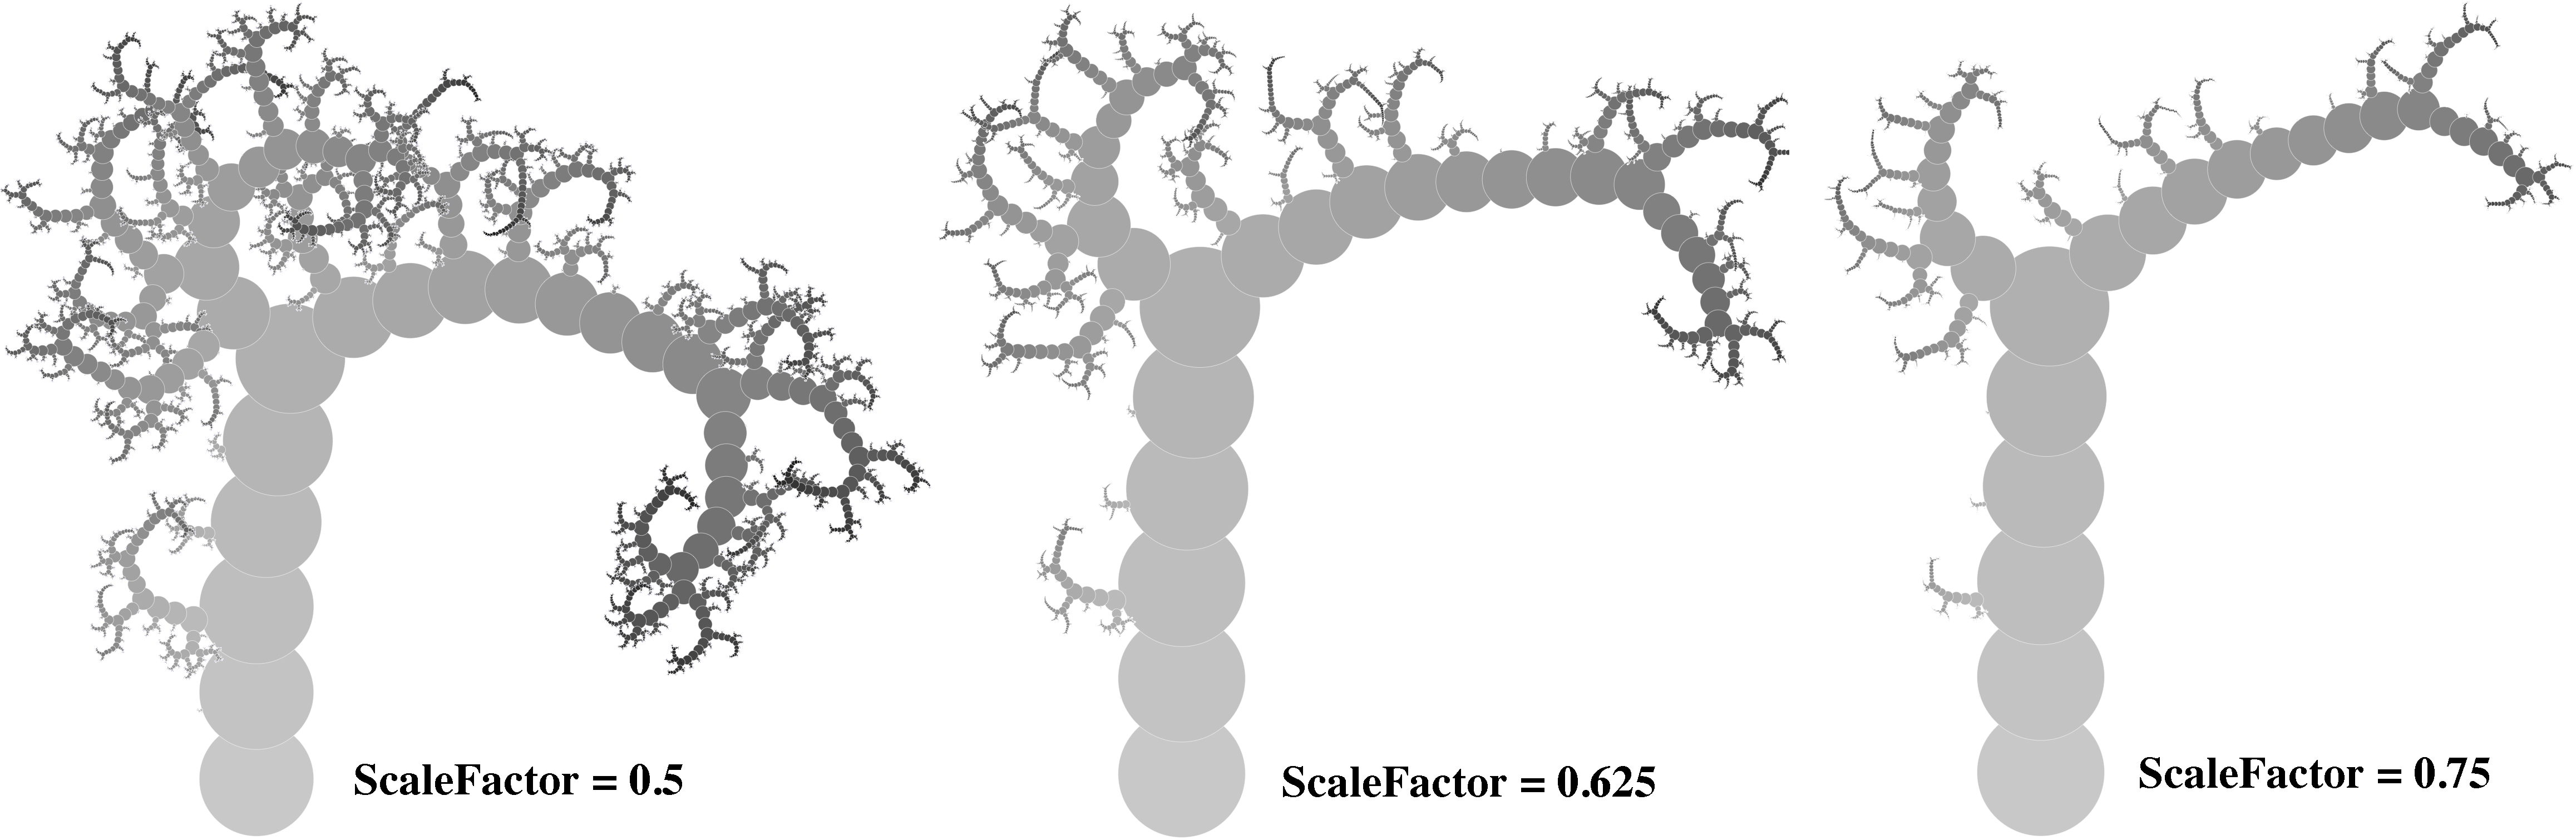
\includegraphics[width=250pt]{figures/UseCase.png}
% \caption{\label{fig:Usecase} \theName{} for the mammal hierarchy with different scales factor in computing node size.}
%\end{figure}


For future work, we plan to conduct more extensive studies of HEB on different tree layouts and to investigate more involved tasks. For instance, we want to explicitly examine a user's understanding of high level inter-cluster connectivity trends by asking the user to identify which cluster/parent node is most strongly connected to a selected cluster/parent node. We also plan to examine user understanding of low level intra-cluster connectivity trends by testing how well a user can identify the connectivity within a cluster/parent node. Additionally, we also plan to explore how interactions, such as rotating, panning, and zooming, support these tasks (especially for deeply nested trees of up to one hundred levels). 

\theName{}~\cite{Dang2017CactusTrees} is implemented in Javascript using the D3.js library~\cite{bostock2011d3}. A demonstration video, the online \theName{} application, and evaluation materials, such as screenshots of techniques the test participants saw, questions they were asked, and the actual user study itself are all available on our project page, located at \url{http://cactustrees.github.io}. 
Examples of complex, real-world datasets discussed in this paper (along with additional datasets) can also be found on our project page, represented both using \theName{} and as compared to a range of other tree layouts.

\section*{Acknowledgements}
This work was funded in part by DARPA under ARO contract W911NF-14-1-0395. 

\bibliographystyle{abbrv}
\bibliography{bibliography}


\end{document}
